\documentclass[a4paper,titlepage]{article}

\makeatletter
\def\input@path{{../../../template/}}
\makeatother

\usepackage{Comandi}
\usepackage{Riferimenti}
\usepackage{Stile}

% -- COMANDI PER I CASI D'USO -- %
\newcommand\UC[1]{\hyperref[#1]{#1}}
\newcommand\Req[1]{\hyperref[#1]{#1}}
\newcommand\boldTitle[1]{\textbf{#1: }}
\newcommand\id[1]{\boldTitle{Identificativo} #1}
\newcommand\tipo{\boldTitle{Tipo}}
\newcommand\tit{\boldTitle{Titolo}}
\newcommand\desc{\boldTitle{Descrizione}}
\newcommand\pre{\boldTitle{Precondizione}}
\newcommand\post{\boldTitle{Postcondizione}}
\newcommand\scen{\boldTitle{Scenario principale}}
\newcommand\scensec{\boldTitle{Scenario secondario}}
\newcommand\att{\boldTitle{Attori}}
\newcommand\ext{\boldTitle{Extension Point}}
\newcommand\casoduso[2]{\subsection{#1 - #2}\label{#1}}
\newcounter{requisitiCounter}
\newcommand\requisito[1]{\refstepcounter{requisitiCounter} \label{#1} #1}

\def\NOME{Analisi dei Requisiti}
\def\VERSIONE{1.0.0}
\def\DATA{2016-04-06}
\def\REDATTORE{Enrico Bellio \\ & Andrea Grendene \\ & Tommaso Panozzo}
\def\VERIFICATORE{Viviana Alessio \\ & Matteo Franco}
\def\RESPONSABILE{Viviana Alessio}
\def\USO{Esterno}
\def\DESTINATARI{\COMMITTENTE \\ & \CARDIN \\ & \PROPONENTE}
\def\SOMMARIO{Descrizione dei Casi d'Uso e l'Analisi dei Requisiti del \gl{progetto}.}

\begin{document}

\maketitle

\begin{diario}
  \modifica{Viviana Alessio}{\RES}{Approvazione documento}{2016-04-06}{1.0.0}
  \modifica{Tommaso Panozzo}{\AN}{Correzione alla verifica generale del documento}{2016-04-03}{0.4.7}
  \modifica{Viviana Alessio}{\VER}{Verifica generale del documento}{2016-04-03}{0.4.6}
  \modifica{Enrico Bellio}{\AN}{Correzioni alla verifica dei requisiti}{2016-04-03}{0.4.5}
  \modifica{Matteo Franco}{\VER}{Verifica dei requisiti}{2016-04-03}{0.4.4}
  \modifica{Andrea Grendene}{\AN}{Correzioni alla seconda verifica dei casi d'uso}{2016-04-03}{0.4.3}
  \modifica{Viviana Alessio}{\VER}{Seconda verifica dei casi d'uso}{2016-04-03}{0.4.2}
  \modifica{Tommaso Panozzo}{\AN}{Correzioni alla prima verifica dei casi d'uso}{2016-04-02}{0.4.1}
  \modifica{Matteo Franco}{\VER}{Prima verifica dei casi d'uso}{2016-04-02}{0.4.0}
  \modifica{Enrico Bellio}{\AN}{Aggiunta diagrammi dei casi d'uso}{2016-03-31}{0.3.0}
  \modifica{Enrico Bellio}{\AN}{Correzioni al testo della descrizione}{2016-03-30}{0.2.8}
  \modifica{Andrea Grendene}{\AN}{Correzioni minori ai requisiti}{2016-03-28}{0.2.7}
  \modifica{Tommaso Panozzo}{\AN}{Correzioni minori ai casi d'uso}{2016-03-28}{0.2.6}
  \modifica{Enrico Bellio}{\AN}{Stesura casi d'uso figli di UC1.6}{2016-03-26}{0.2.5}
  \modifica{Tommaso Panozzo}{\AN}{Stesura requisiti derivati da UC1.3}{2016-03-26}{0.2.4}
  \modifica{Andrea Grendene}{\AN}{Stesura casi d'uso figli di UC1.3}{2016-03-24}{0.2.3}
  \modifica{Enrico Bellio}{\AN}{Stesura preliminare delle sezioni di descrizione}{2016-03-24}{0.2.2}
  \modifica{Andrea Grendene}{\AN}{Stesura dei primi requisiti}{2016-03-24}{0.2.1}
  \modifica{Tommaso Panozzo}{\AN}{Stesura dei primi casi d'uso}{2016-03-24}{0.2.0}
  \modifica{Andrea Grendene}{\AN}{Modifiche minori alla struttura}{2016-03-22}{0.1.1}
  \modifica{Tommaso Panozzo}{\AN}{Stesura struttura documento}{2016-03-18}{0.1.0}
\end{diario}

\newpage
\tableofcontents
\newpage
\listoftables
\newpage
\listoffigures

\newpage
\section{Introduzione}
	\subsection{Scopo del documento} 
	Questo documento ha lo scopo di spiegare dettagliatamente le strategie secondo cui il gruppo \AUTORE{} intende condurre il \gl{progetto} didattico. 
	\subsection{Scopo del \gl{prodotto}}
	\SCOPO
	\subsection{Glossario}
	\GLOSSARIO
	\subsection{Riferimenti}
		\subsubsection{Normativi}
			\begin{itemize}
				\item \textbf{Capitolato d'appalto C2 - CLIPS:} Communication \& Localisation with Indoor Positioning Systems. \\
				\url{http://www.math.unipd.it/~tullio/IS-1/2015/Progetto/C2.pdf}
				\item \textbf{Vincoli e dettagli tecnico-economici} \\
				\url{http://www.math.unipd.it/~tullio/IS-1/2015/Dispense/PD01.pdf}
				\item \textbf{Norme di Progetto} \\ \NPdoc
				\item \textbf{Regolamento di Progetto} \\
				\url{http://www.math.unipd.it/~tullio/IS-1/2015/Progetto/}
				\item \textbf{Regolamento organigramma} \\
				\url{http://www.math.unipd.it/~tullio/IS-1/2015/Progetto/PD01b.html}
			\end{itemize}	
			
		\subsubsection{Informativi}
			\begin{itemize}
				\item \textbf{Software Engineering (10th edition}) \\
				Ian Sommerville \\
				Pearson Education | Addison-Wesley
				\item \textbf{Guide to the Software Engineering Body of Knowledge}
				IEEE Computer Society. Software Engineering Coordinating Committee
				\item \textbf{Slides del \COMMITTENTE} \\ riguardo i  \href{http://www.math.unipd.it/~tullio/IS-1/2015/Dispense/L02.pdf}{processi \gl{software}}, il \href{http://www.math.unipd.it/~tullio/IS-1/2015/Dispense/L03.pdf}{ciclo di vita del \gl{software}} e \href{http://www.math.unipd.it/~tullio/IS-1/2015/Dispense/L04.pdf}{la gestione di \gl{progetto}}	
			\end{itemize}
	\subsection{Modello di ciclo di vita scelto}
	È stato scelto come ciclo di vita il modello \gl{incrementale}. Le motivazioni che ci hanno spinto verso questa direzione sono il modo in cui è strutturato il \gl{progetto} didattico e la quasi totale inesperienza dei componenti del gruppo nello sviluppare progetti \gl{software} di grandi dimensioni. Di seguito una lista di caratteristiche del metodo \gl{incrementale}:
	\begin{itemize}
		\item si può produrre valore ad ogni incremento;
		\item ogni incremento riduce il rischio di fallimento;
		\item prevede rilasci multipli;
		\item i requisiti utente sono classificati e trattati in base alla loro importanza strategica. I requisiti più importanti sono già stabili all'inizio dello sviluppo del \gl{progetto};
		\item l'analisi dei requisiti e la progettazione architetturale non vengono ripetute;
		\item prima si pensa allo sviluppo dei requisiti essenziali, poi a quelli desiderabili;
		\item Sono presenti delle iterazioni del tipo Prototipo $\rightarrow$ Validazione $\rightarrow$ Prototipo $\rightarrow$ Validazione $\rightarrow$ ecc..
	\end{itemize}
	\subsection{Scadenze}
	Il gruppo Beacon Strips ha deciso di rispettare le seguenti scadenze:
	\begin{itemize} 
		\item \textbf{Revisione dei Requisiti}: 2016-04-18
		\item \textbf{Revisione di Progettazione}: 2016-06-17
		\item \textbf{Revisione di Qualifica}: 2016-08-24
		\item \textbf{Revisione di Accettazione}: 2016-09-12
	\end{itemize}
	In base a queste scadenze e a fronte dell'analisi dei rischi verranno decise le fasi in cui suddividere il lavoro di sviluppo del \gl{progetto}.
	\subsubsection{Scelta Revisione di Progettazione}
	Si è deciso di affrontare la RP$_{\mbox{\textit{min}}}$. Il gruppo si impegna quindi per il 2016-06-17 di presentare nel documento ``Specifica Tecnica'' la progettazione ad alto livello del \gl{prodotto}.
	

\newpage
\section{Descrizione Generale}
\label{sec:DescrizioneGenerale}

\subsection{Obbiettivi del prodotto}
\label{sec:ObbiettiviDelProdotto}
Il prodotto ha come scopo principale la creazione di un'applicazione che possa intrattenere l'utente grazie all'utilizzo dei beacons. Nello specifico l'applicazione condurrà l'utente a percorrere un determinato percorso grazie alla ricerca del giusto beacon e alla risoluzione del semplice gioco o indovinello ad esso associato.

\subsection{Funzioni del Prodotto}



\newpage
\label{sec:CasiUso}
\section{Casi d'Uso}
\label{sec:CasiUso}
Gli Analisti dopo aver discusso, aver analizzato il \gl{capitolato} d'appalto e grazie agli incontri con il Proponente hanno definito i seguenti casi d'uso.
Ogni caso d'uso ha la seguente forma:
\begin{center}
	UC[codice identificativo del padre].[codice progressivo di livello]
\end{center}
il codice progressivo può includere più livelli di gerarchia separati da un punto.
\casoduso{UC1}{Login}
\begin{figure}[H]
\centering
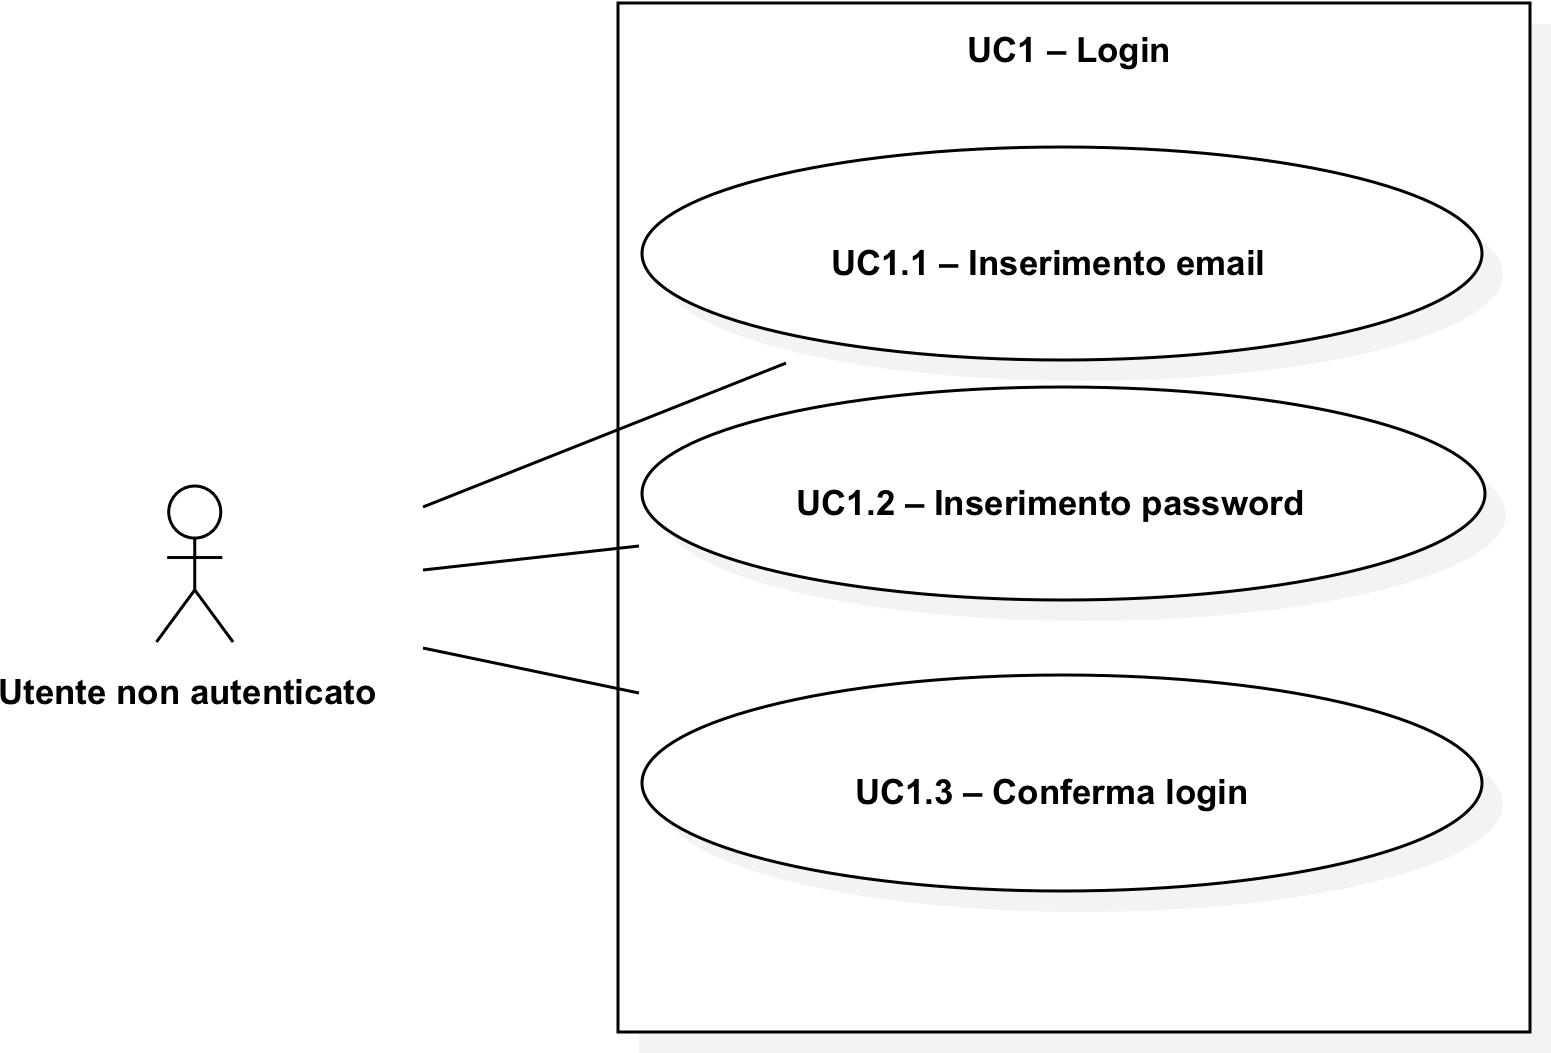
\includegraphics[scale=0.2]{img/UC1.png}
\caption{Caso d'uso UC1 - Login}
 \end{figure}
\desc{l'utente effettua il login con le proprie credenziali.}\\\\
\pre{l'utente è registrato presso il database.}\\\\
\post{l'utente è autenticato.}\\\\
\scen{\begin{itemize}
\item \UC{UC1.1} l'utente inserisce l'email;
\item \UC{UC1.2} l'utente inserisce la password;
\item \UC{UC1.3} l'utente conferma di voler eseguire il login.
\end{itemize}}\\\\
\scensec{\begin{itemize}
\item ESTENSIONE: se i dati inseriti non sono corretti l'esecuzione prosegue con \UC{UC14};
\item ESTENSIONE: se l'utente non ricorda le proprie credenziali di accesso può recuperarle grazie a \UC{UC20}.
\end{itemize}}\\\\
\att{Utente non autenticato.}

\casoduso{UC1.1}{Inserimento email}
\desc{l'utente inserisce l'indirizzo email con cui si è registrato in precedenza.}\\\\
\pre{la connessione ad internet è attiva e l'app fornisce la pagina di login.}\\\\
\post{l'utente ha inserito la mail.}\\\\
\scen{l'utente inserisce l'indirizzo email con cui si è registrato in precedenza.}\\\\
\att{Utente non autenticato.}

\casoduso{UC1.2}{Inserimento password}
\desc{l'utente inserisce la password con cui si è registrato in precedenza rispettando il requisito \Req{R0F1.2.7.3}.}\\\\
\pre{la connessione ad internet è attiva e l'app fornisce la pagina di login.}\\\\
\post{l'utente ha inserito la password.}\\\\
\scen{l'utente inserisce la password con cui si è registrato in precedenza rispettando il requisito \Req{R0F1.2.7.3}.}\\\\
\att{Utente non autenticato.}

\casoduso{UC1.3}{Conferma Login}
\desc{l'utente conferma di voler procedere con l'autenticazione con i dati precedentemente inseriti.}\\\\
\pre{la connessione ad internet è attiva e l'app fornisce la pagina di login.}\\\\
\post{l'utente è stato autenticato.}\\\\
\scen{l'utente conferma di voler procedere con l'autenticazione con i dati precedentemente inseriti.}\\\\
\att{Utente non autenticato.}

\casoduso{UC2}{Deautenticazione}
\desc{l'utente autenticato esegue il logout.}\\\\
\pre{l'utente è autenticato.}\\\\
\post{l'utente non è più autenticato.}\\\\
\scen{l'utente autenticato esegue il logout.}\\\\
\att{Utente autenticato.}

\casoduso{UC3}{Svolgimento del percorso}
\begin{figure}[H]
\centering
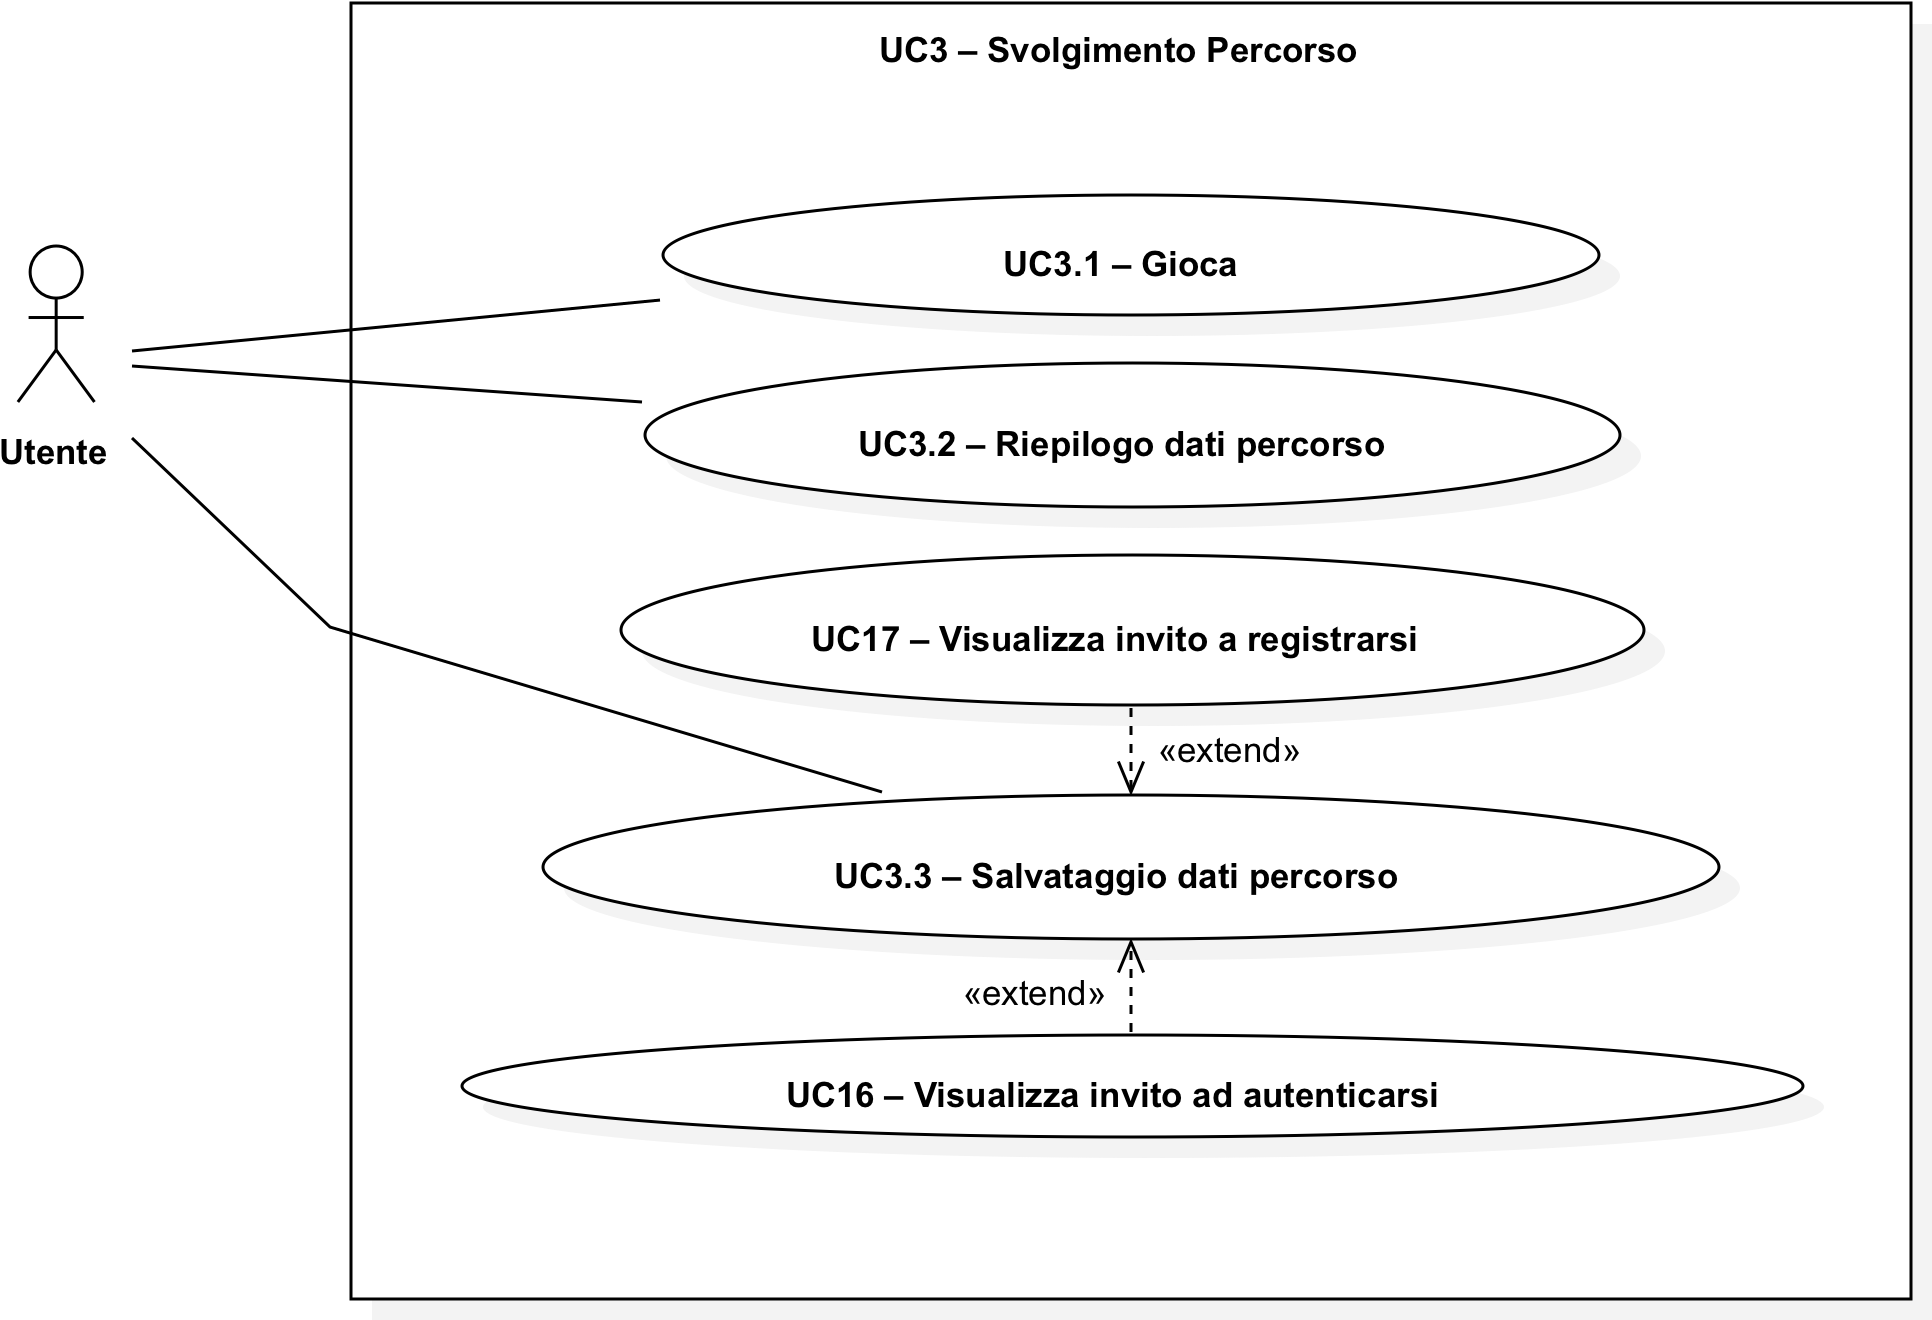
\includegraphics[scale=0.2]{img/UC3.png}
\caption{Caso d'uso UC3 - Svolgimento del percorso}
 \end{figure}
\desc{l'utente svolge un percorso tra quelli disponibili nel luogo in cui si trova.}\\\\
\pre{l'utente ha i servizi di localizzazione, il Bluetooth e la connessione ad internet attivi e si trova in un luogo abilitato.}\\\\
\post{l'utente ha completato il percorso selezionato.}\\\\
\scen{l'utente effettua i seguenti passi:
\begin{itemize}
\item \UC{UC3.1} l'utente gioca il percorso;
\item \UC{UC3.2} l'utente visualizza i dati del percorso appena concluso;
\item \UC{UC3.3} l'utente autenticato salva i risultati.
\end{itemize}}\\\\
\att{Utente.}

\casoduso{UC3.1}{Gioca}
\begin{figure}[H]
\centering
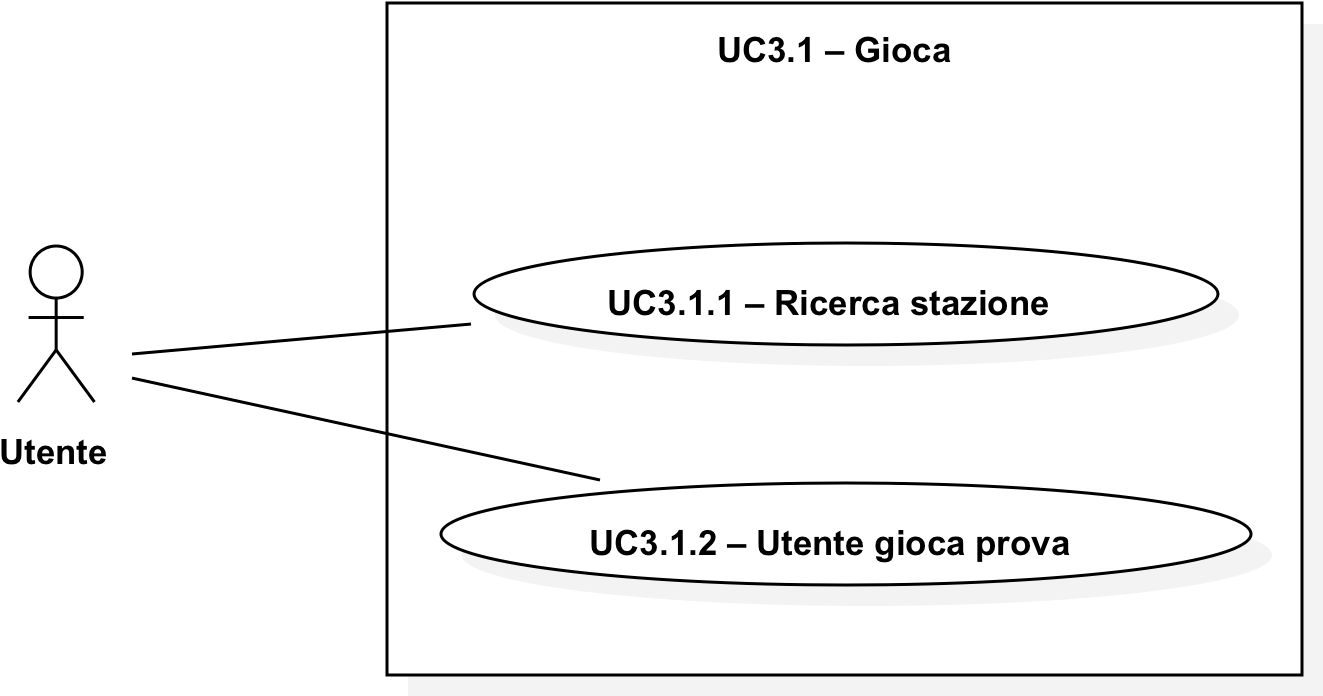
\includegraphics[scale=0.2]{img/UC3_1.png}
\caption{Caso d'uso UC3.1 - Gioca}
 \end{figure}
\desc{l'utente si trova in un luogo abilitato, scarica un percorso e lo conclude.}\\\\
\pre{l'utente ha scelto un percorso.}\\\\
\post{l'utente completa tutte le prove.}\\\\
\scen{\begin{itemize}
\item \UC{UC3.1.1} l'utente ricerca una stazione;
\item \UC{UC3.1.2} l'utente svolge la prova della stazione in cui si trova.
\end{itemize}}\\\\
\att{Utente.}

\casoduso{UC3.1.1}{Ricerca stazione}
\desc{l'utente è alla ricerca della stazione in cui recarsi per la prossima o la prima prova.}\\\\
\pre{l'utente non sta svolgendo alcuna prova e non ha concluso il percorso.}\\\\
\post{l'utente è presso la stazione in cui svolgere la prossima prova.}\\\\
\scen{l'utente è alla ricerca della stazione in cui recarsi per la prossima o la prima prova.}\\\\
\att{Utente.}

\casoduso{UC3.1.2}{Utente gioca prova}
\begin{figure}[H]
\centering
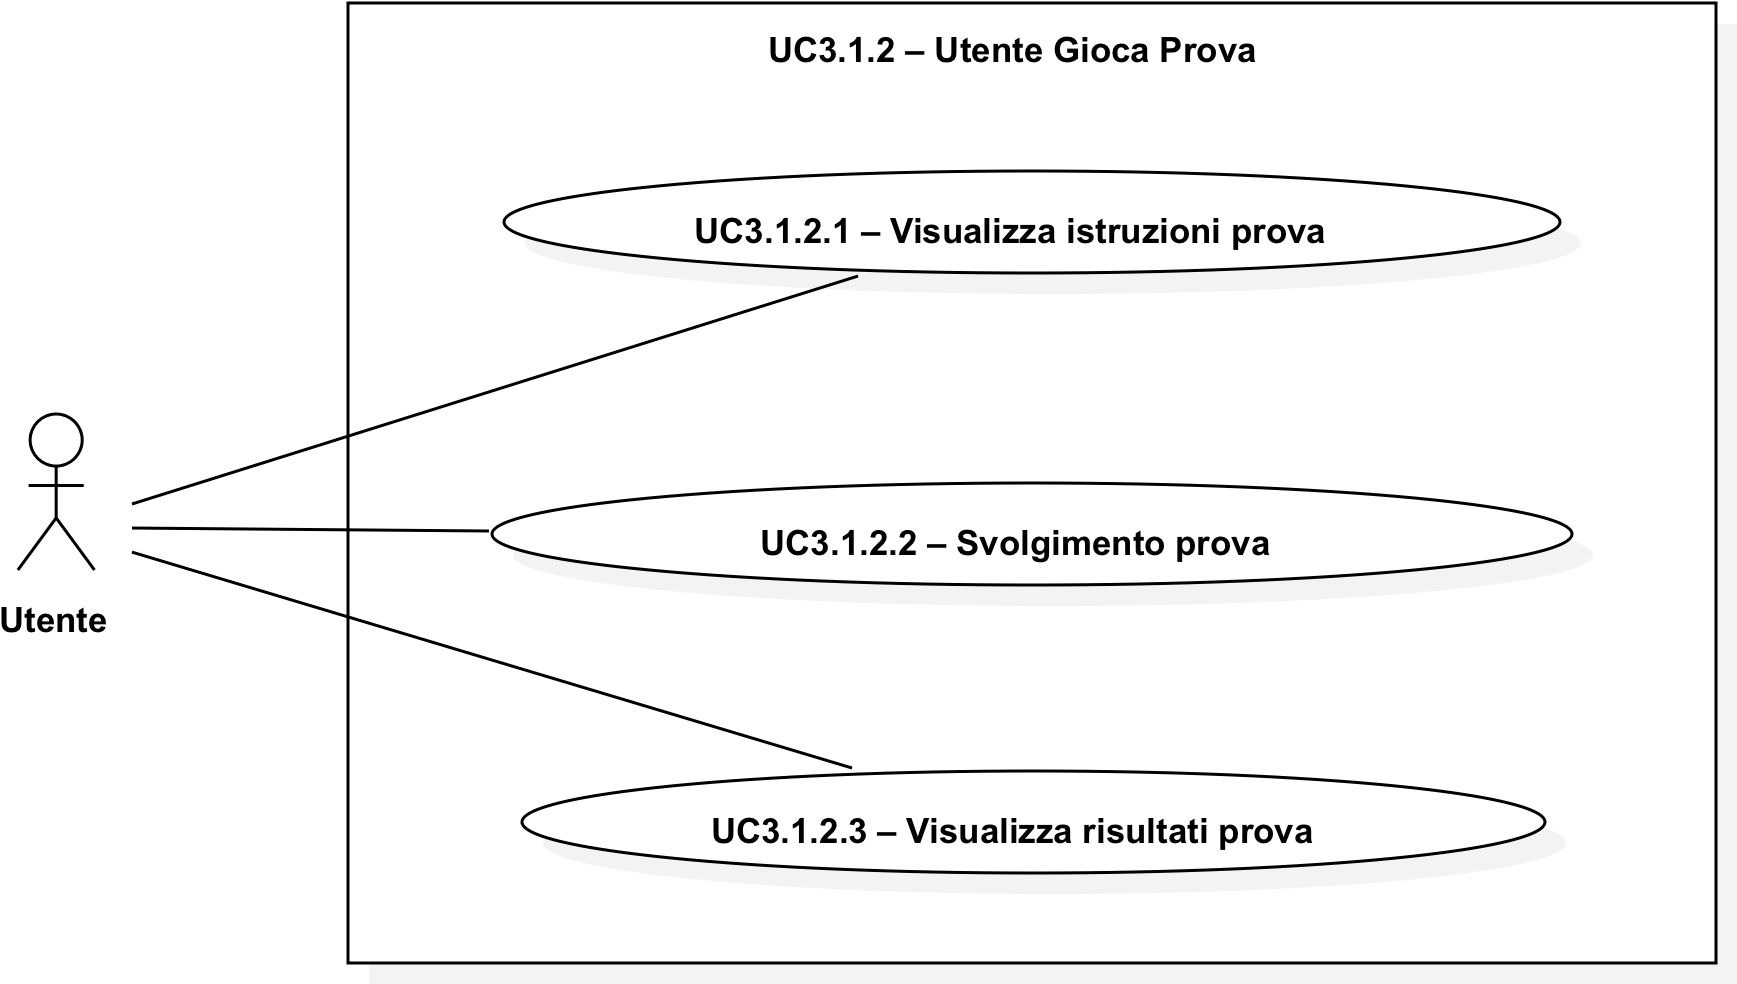
\includegraphics[scale=0.2]{img/UC3_1_2.png}
\caption{Caso d'uso UC3.1.2 - Utente gioca prova}
 \end{figure}
\desc{l'utente affronta la prova della stazione in cui si trova.}\\\\
\pre{l'utente si trova nella sua prossima stazione.}\\\\
\post{l'utente ha completato la prova.}\\\\
\scen{\begin{itemize}
\item \UC{UC3.1.2.1} l'utente visualizza una descrizione della prova;
\item \UC{UC3.1.2.2} l'utente gioca la prova;
\item \UC{UC3.1.2.3} l'utente ottiene un punteggio sulla prova.
\end{itemize}}\\\\
\att{Utente.}

\casoduso{UC3.1.2.1}{Visualizza istruzioni prova}
\desc{l'utente visualizza le informazioni che deve sapere in preparazione alla prova, solitamente le istruzioni (il tempo per la prova non scorre ancora).}\\\\
\pre{l'utente è in procinto di iniziare la prova.}\\\\
\post{l'utente ha ricevuto informazioni su come procedere per la prova.}\\\\
\scen{l'utente visualizza le informazioni che deve sapere in preparazione alla prova, solitamente le istruzioni (il tempo per la prova non scorre ancora).}\\\\
\att{Utente.}

\casoduso{UC3.1.2.2}{Svolgimento prova}
\desc{l'utente svolge la prova prevista per la stazione.}\\\\
\pre{l'utente ha visualizzato le informazioni necessarie allo svolgimento della prova.}\\\\
\post{l'utente ha concluso la prova con successo.}\\\\
\scen{l'utente svolge la prova prevista per la stazione.}\\\\
\att{Utente.}

\casoduso{UC3.1.2.3}{Visualizza risultati prova}
\desc{l'utente viene informato circa i risultati ottenuti durante la prova appena conclusa.}\\\\
\pre{l'utente ha appena concluso una prova.}\\\\
\post{l'utente ha ottenuto i risultati circa la prova appena conclusa.}\\\\
\scen{l'utente viene informato circa i risultati ottenuti durante la prova appena conclusa.}\\\\
\att{Utente.}

\casoduso{UC3.2}{Riepilogo dati
percorso}
\begin{figure}[H]
\centering
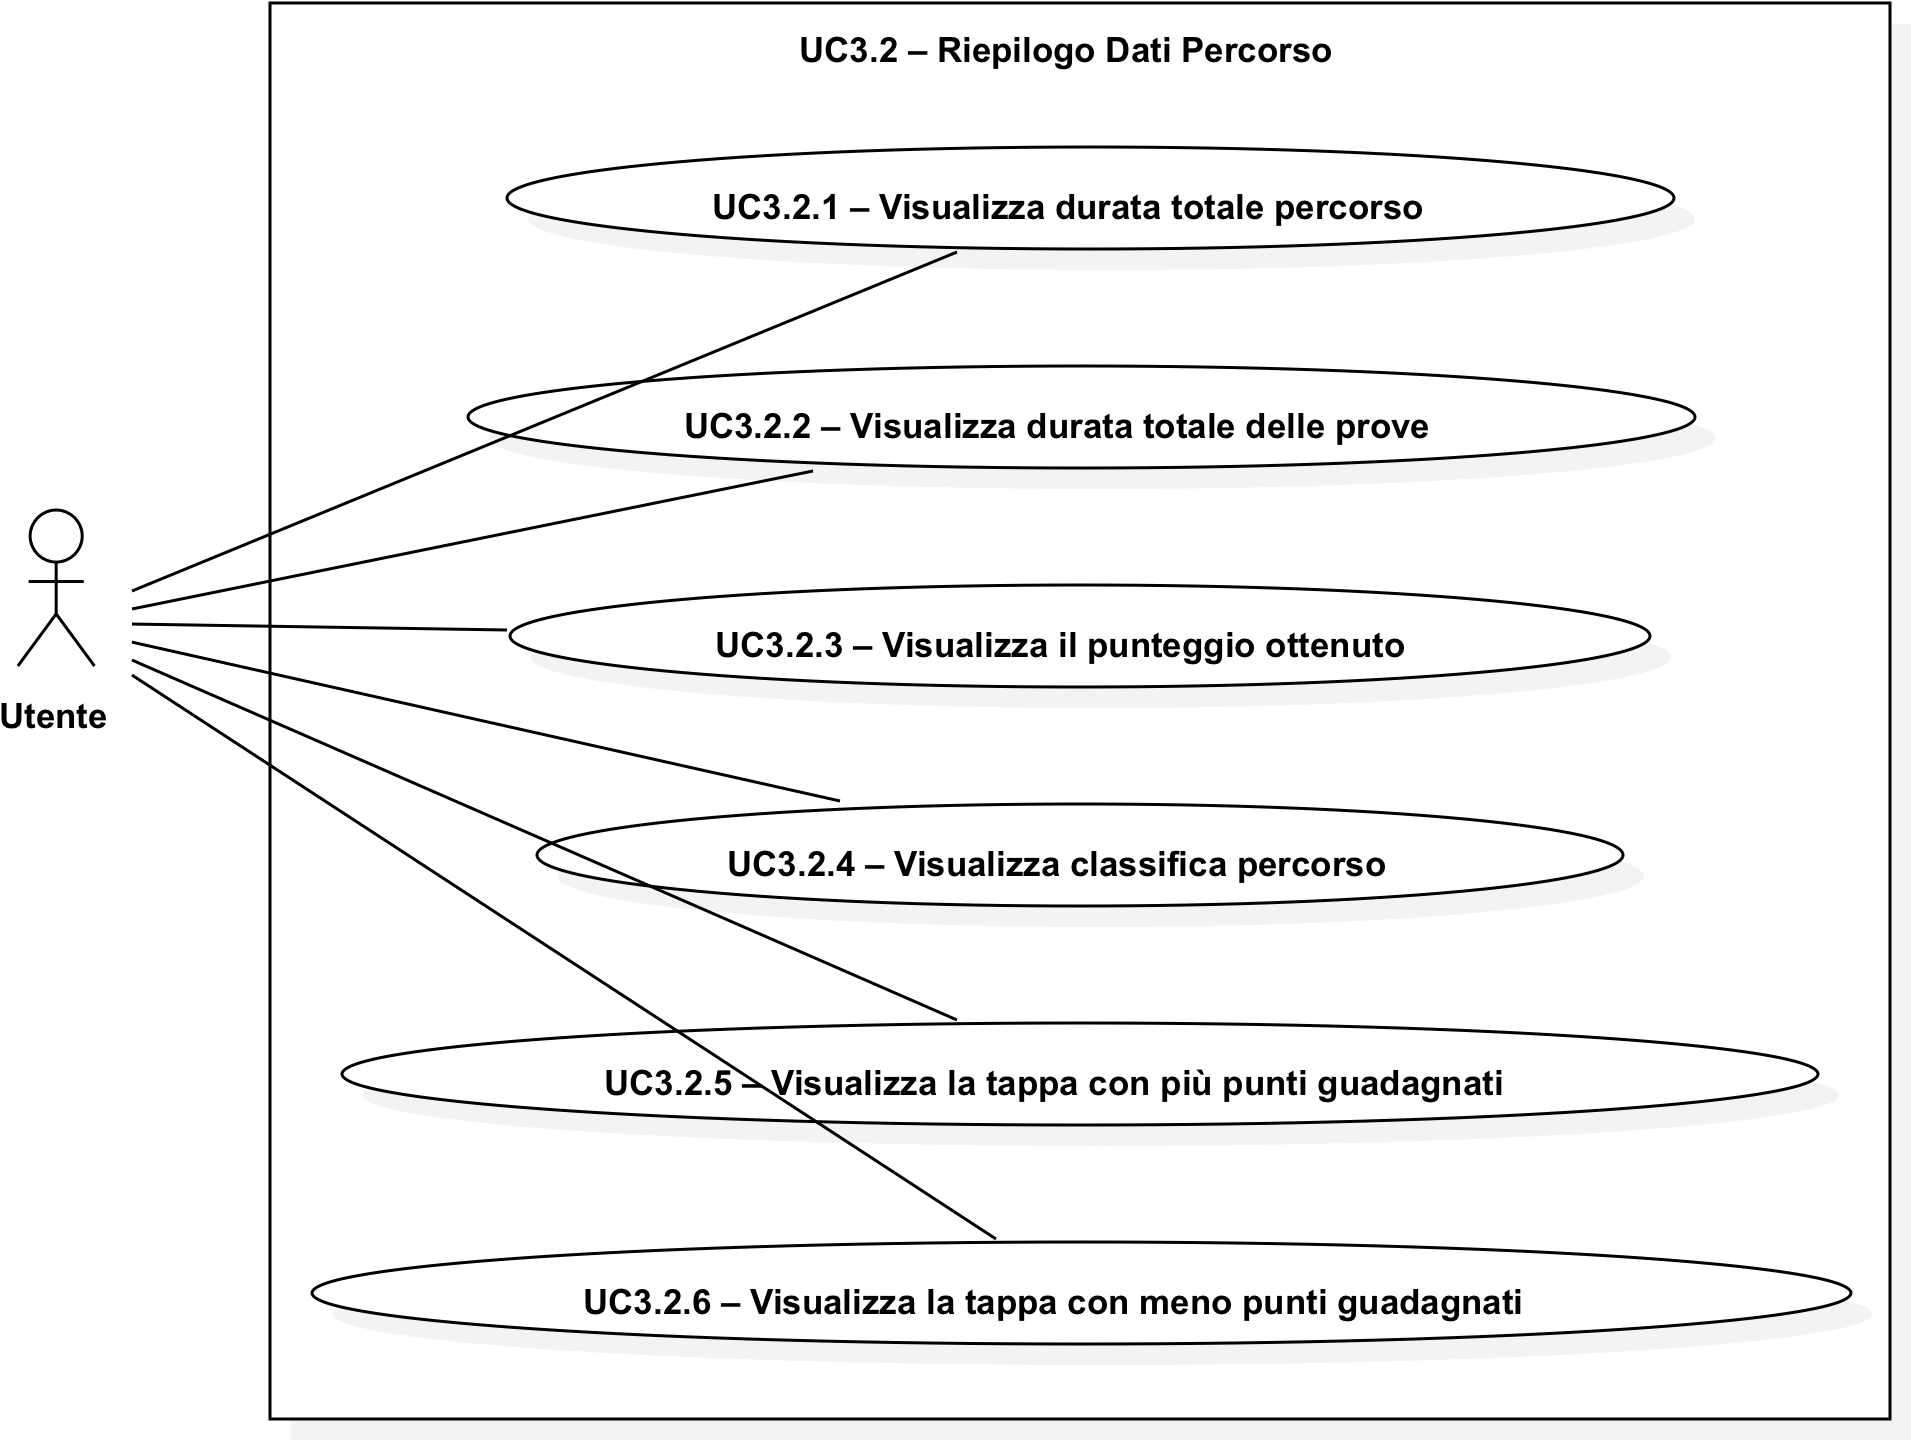
\includegraphics[scale=0.2]{img/UC3_2.png}
\caption{Caso d'uso UC3.2 - Riepilogo dati percorso}
 \end{figure}
\desc{dopo che l'utente termina il percorso visualizza il riassunto: durata totale, durata totale delle prove, punteggio ottenuto, posizione in classifica.}\\\\
\pre{l'utente ha completato il percorso.}\\\\
\post{l'utente ha visualizzato il riassunto del percorso.}\\\\
\scen{L'utente visualizza le seguenti informazioni:
\begin{itemize}
 \item \UC{UC3.2.1} informazioni generali sulla durata (orario di inizio/fine, durata totale);
\item \UC{UC3.2.2} durata delle prove (somma della durata di ciascuna prova);
\item \UC{UC3.2.3} punteggio ottenuto (somma dei punteggi ottenuti nelle varie prove);
\item \UC{UC3.2.4} punteggio medio ottenuto dagli utenti (media dei punteggi ottenuti su quel percorso);
\item \UC{UC3.2.5} visualizza la tappa in cui è stato ottenuto il maggior numero di punti;
\item \UC{UC3.2.6} visualizza la tappa in cui è stato ottenuto il minor numero di punti.
\end{itemize}}\\\\
\att{Utente.}

\casoduso{UC3.2.1}{Visualizza durata totale percorso}
\desc{l'utente visualizza il tempo totale impiegato per il percorso, ovvero il tempo intercorso tra l'orario di inizio e quello di fine.}\\\\
\pre{l'utente ha concluso il percorso.}\\\\
\post{l'app mostra i dettagli sul tempo di inizio, fine e durata.}\\\\
\scen{l'utente visualizza il tempo totale impiegato per il percorso, ovvero il tempo intercorso tra l'orario di inizio e quello di fine.}\\\\
\att{Utente.}

\casoduso{UC3.2.2}{Visualizza durata totale delle prove}
\desc{l'utente visualizza la durata totale del percorso: la somma dei tempi spesi dall'utente nel compiere le varie prove.}\\\\
\pre{l'utente ha concluso il percorso.}\\\\
\post{l'utente ha visualizzato i dettagli sulla durata delle prove.}\\\\
\scen{l'utente visualizza la durata totale del percorso: la somma dei tempi spesi dall'utente nel compiere le varie prove.}\\\\
\att{Utente.}

\casoduso{UC3.2.3}{Visualizza il punteggio ottenuto}
\desc{l'utente visualizza il punteggio ottenuto durante il percorso che è composto dalla somma dei punteggi ottenuti nelle varie prove.}\\\\
\pre{l'utente ha concluso il percorso.}\\\\
\post{l'utente ha visualizzato il punteggio ottenuto.}\\\\
\scen{l'utente visualizza il punteggio ottenuto durante il percorso che è composto dalla somma dei punteggi ottenuti nelle varie prove.}\\\\
\att{Utente.}

\casoduso{UC3.2.4}{Visualizza classifica del percorso}
\desc{l'utente visualizza alcune informazioni circa le prime posizioni in classifica, quelle antecedenti e quelle seguenti l'utente nel percorso appena concluso (si veda \Req{R0F3.2.4} e figli).}\\\\
\pre{l'utente ha concluso il percorso.}\\\\
\post{l'utente ha visualizzato la sua posizione in classifica assoluta ottenuta per quel percorso.}\\\\
\scen{l'utente visualizza alcune informazioni circa le prime posizioni in classifica, quelle antecedenti e quelle seguenti l'utente nel percorso appena concluso (si veda \Req{R0F3.2.4} e figli).}\\\\
\att{Utente.}

\casoduso{UC3.2.5}{Visualizza la tappa con più punti guadagnati}
\desc{l'utente visualizza la tappa del percorso appena concluso dove ha accumulato il maggior numero di punti.}\\\\
\pre{l'utente ha concluso il percorso.}\\\\
\post{l'utente ha visualizzato la prova in cui ha accumulato il maggior numero di punti.}\\\\
\scen{l'utente visualizza la tappa del percorso appena concluso dove ha accumulato il maggior numero di punti.}\\\\
\att{Utente.}

\casoduso{UC3.2.6}{Visualizza la tappa con meno punti guadagnati}
\desc{l'utente visualizza la tappa del percorso appena concluso in cui l'utente ha accumulato il minor numero di punti.}\\\\
\pre{l'utente ha concluso il percorso.}\\\\
\post{l'utente ha visualizzato la prova in cui ha accumulato il minor numero di punti.}\\\\
\scen{l'utente visualizza la tappa del percorso appena concluso in cui l'utente ha accumulato il minor numero di punti.}\\\\
\att{Utente.}

\casoduso{UC3.3}{Salvataggio dati percorso}
\desc{l'utente autenticato può salvare i dati relativi al percorso appena conclusosi.}\\\\
\pre{si è concluso il percorso, l'utente è autenticato.}\\\\
\post{i dati del percorso vengono salvati nel database per una futura consultazione.}\\\\
\scen{l'utente autenticato può salvare i dati relativi al percorso appena conclusosi.}\\\\
\scensec{ESTENSIONE: \begin{itemize}
\item \UC{UC16} l'utente non è autenticato e visualizza l'invito ad autenticarsi per salvare i dati del percorso;
\item \UC{UC17} l'utente visualizza l'invito a registrarsi per poi autenticarsi e salvare i dati del percorso.
\end{itemize}}\\\\
\att{Utente.}

\casoduso{UC4}{Visualizza informazioni e contatti utili}
\begin{figure}[H]
\centering
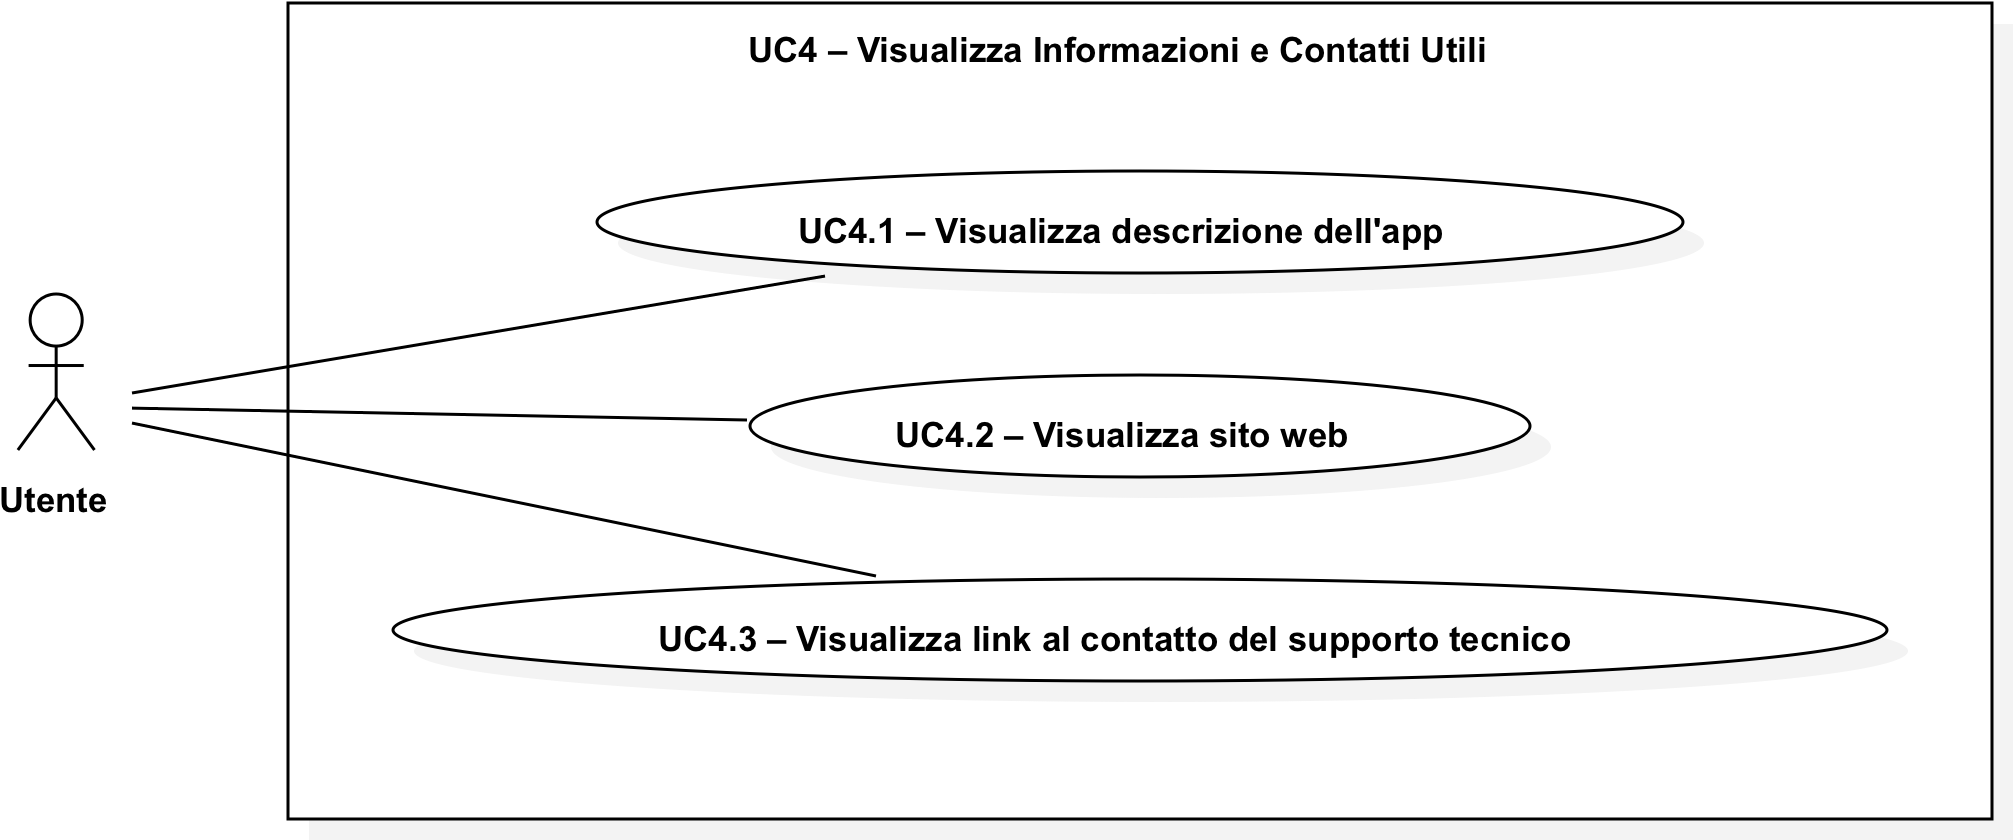
\includegraphics[scale=0.2]{img/UC4.png}
\caption{Caso d'uso UC4 - Visualizza informazioni e contatti utili}
 \end{figure}
\desc{l'utente visualizza le informazioni relative all'app.}\\\\
\pre{l'utente ha l'app installata e in esecuzione.}\\\\
\post{l'utente si è informato riguardo l'app.}\\\\
\scen{\begin{itemize}
\item \UC{UC4.1} l'utente visualizza una descrizione delle funzionalità dell'app;
\item \UC{UC4.2} l'utente visita il sito web dell'app;
\item \UC{UC4.3} l'utente visualizza il contatto al supporto tecnico dell'app.
\end{itemize}}\\\\
\att{Utente.}

\casoduso{UC4.1}{Visualizza descrizione dell'app}
\desc{l'utente visualizza una schermata con un testo esplicativo delle funzionalità dell'app.}\\\\
\pre{l'utente ha l'app installata e in esecuzione.}\\\\
\post{l'utente ha visualizzato la descrizione delle funzionalità dell'app.}\\\\
\scen{l'utente visualizza una schermata con un testo esplicativo delle funzionalità dell'app.}\\\\
\att{Utente.}

\casoduso{UC4.2}{Visualizza sito Web}
\desc{l'utente visualizza il sito web relativo all'app per ottenere maggiori informazioni a riguardo.}\\\\
\pre{l'utente è nella pagina di visualizzazione delle informazioni e dei contatti utili.}\\\\
\post{l'utente ha visualizzato il sito web relativo all'app tramite il browser del dispositivo.}\\\\
\scen{l'utente visualizza il sito web relativo all'app per ottenere maggiori informazioni a riguardo.}\\\\
\att{Utente.}

\casoduso{UC4.3}{Visualizza link di contatto al supporto tecnico dell'app}
\desc{si apre il client email di default nel dispositivo con il campo destinatario impostato all'indirizzo di supporto dell'app per inviare una segnalazione al supporto tecnico.}\\\\
\pre{l'utente ha riscontrato un mal funzionamento dell'app.}\\\\
\post{l'utente è stato indirizzato al client email di default del dispositivo per inviare una segnalazione al supporto tecnico.}\\\\
\scen{si apre il client email di default nel dispositivo con il campo destinatario impostato all'indirizzo di supporto dell'app per inviare una segnalazione al supporto tecnico.}\\\\
\att{Utente.}

\casoduso{UC5}{Cambio credenziali d'accesso}
\begin{figure}[H]
\centering
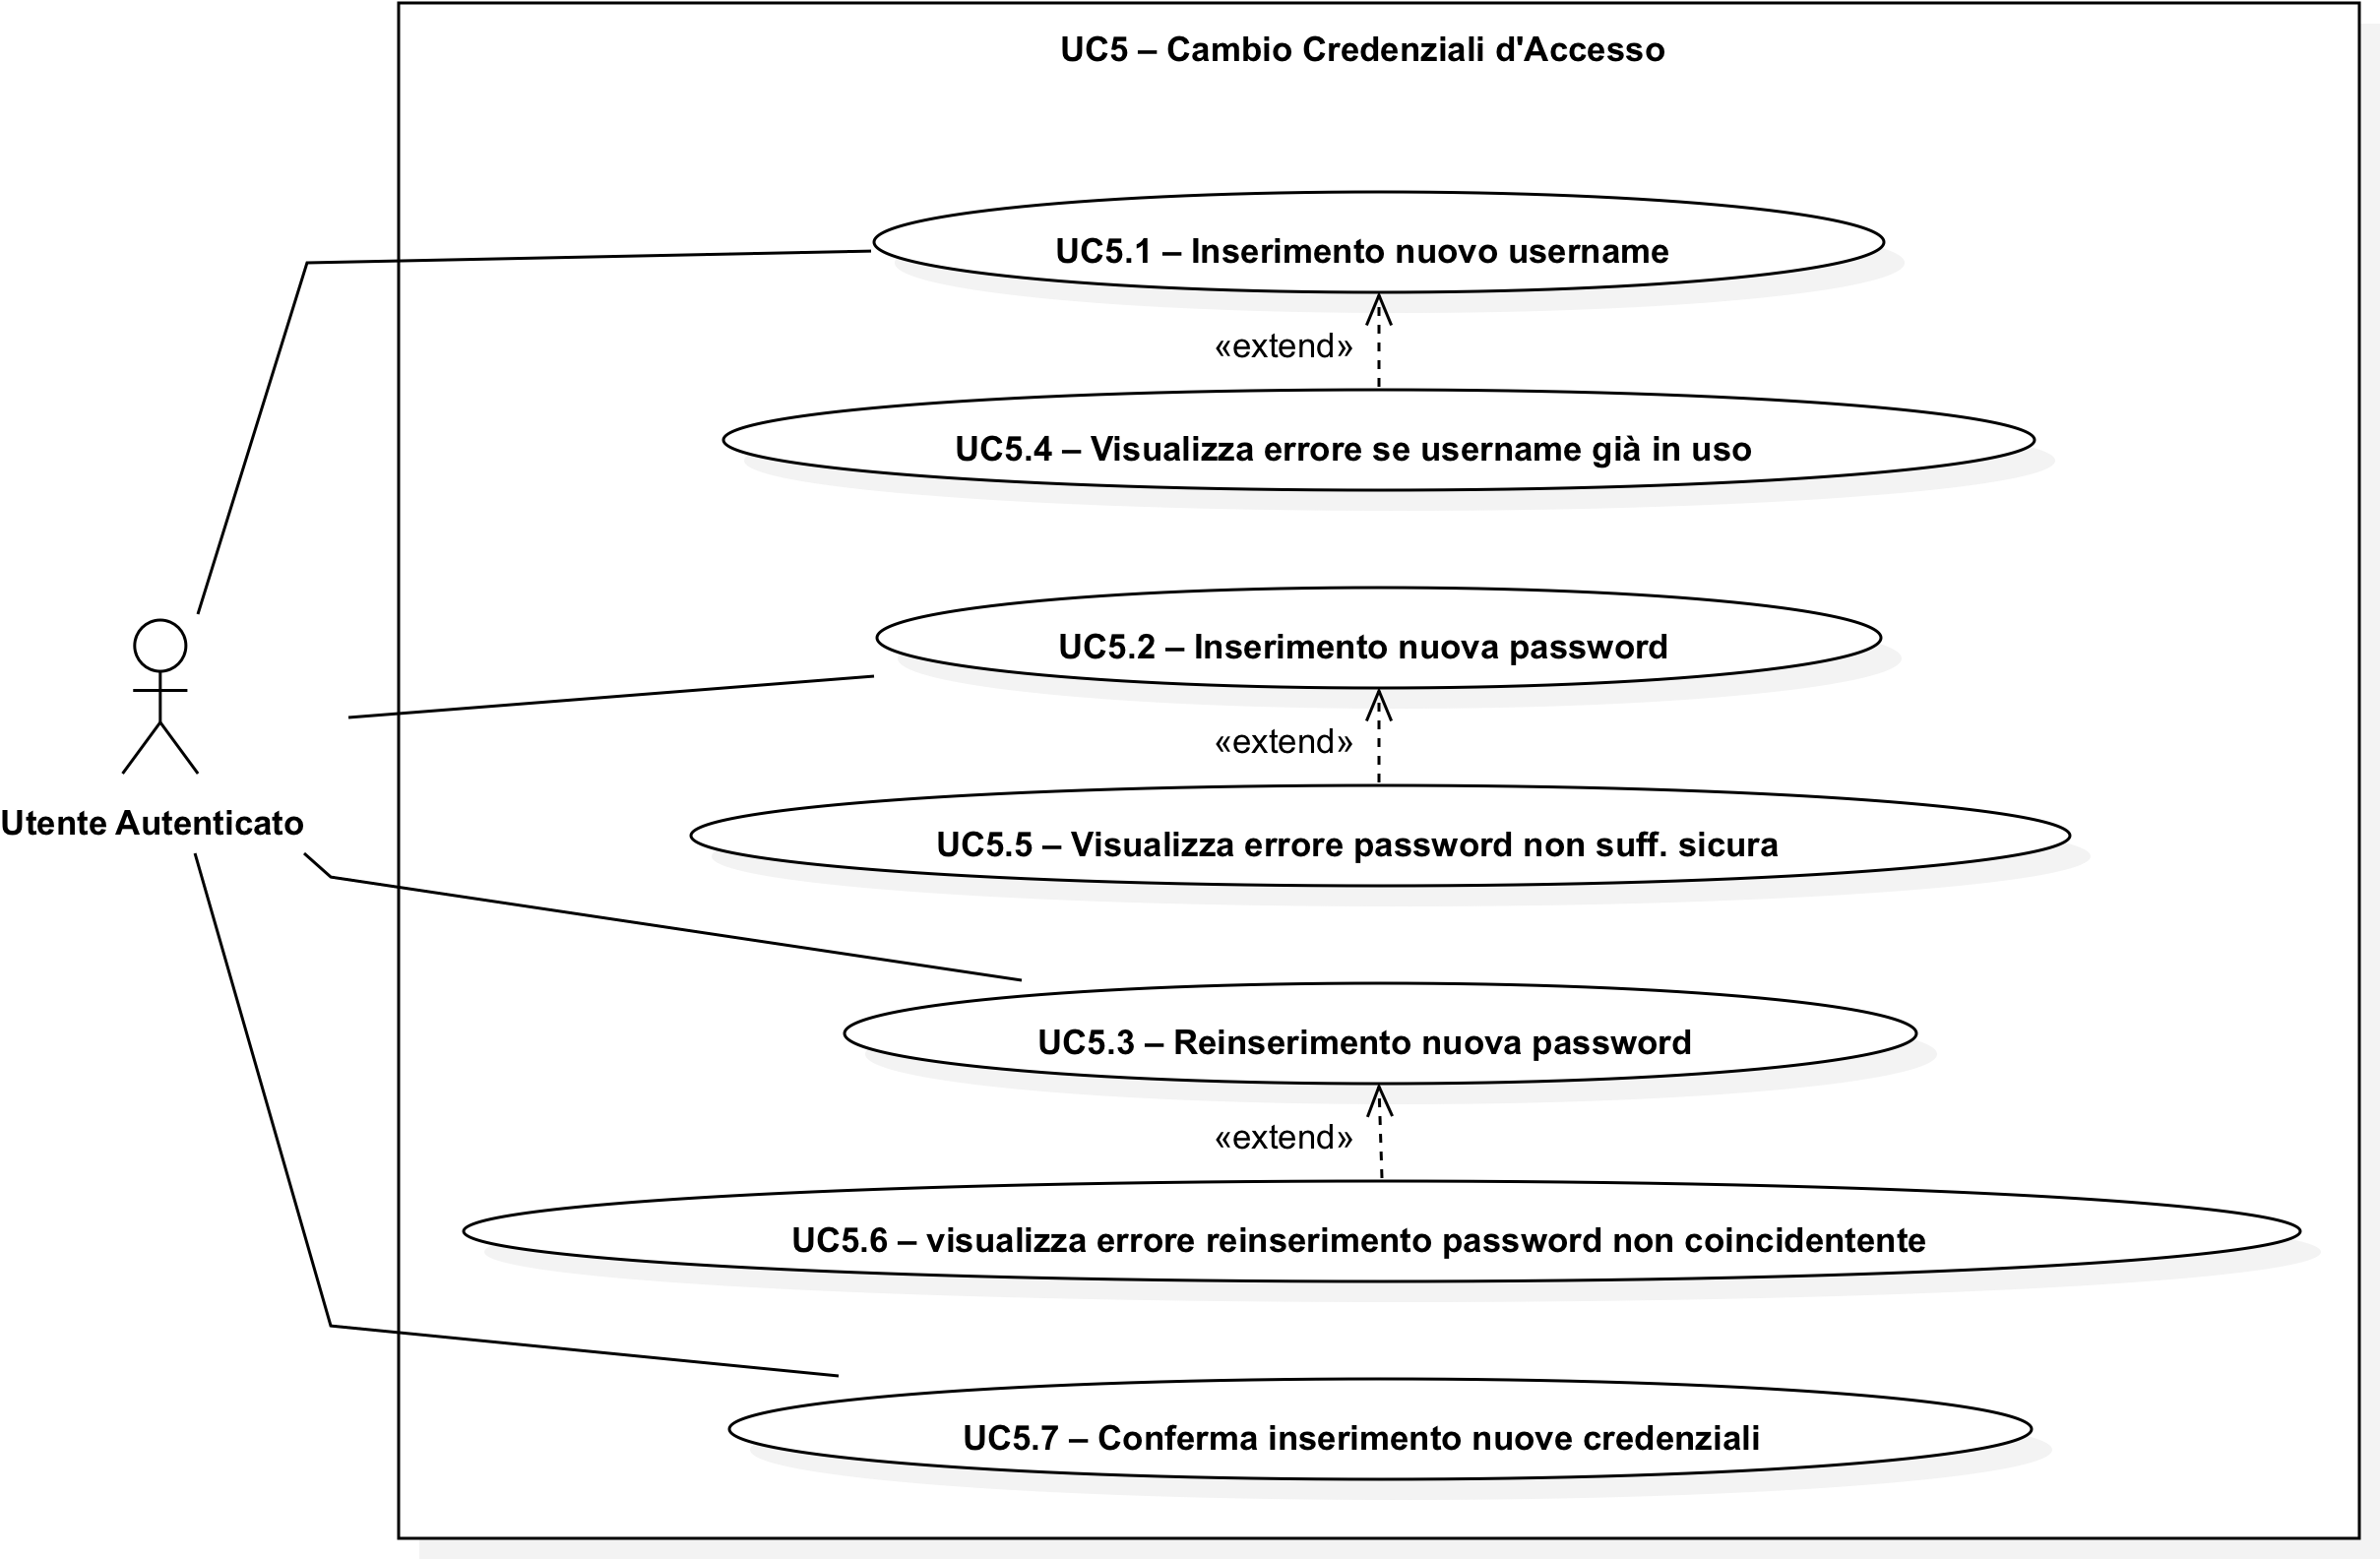
\includegraphics[scale=0.2]{img/UC5.png}
\caption{Caso d'uso UC5 - Cambio credenziali d'accesso}
 \end{figure}
\desc{l'utente modifica le credenziali d'accesso.}\\\\
\pre{l'utente è autenticato.}\\\\
\post{l'utente ha modificato una o più credenziali d'accesso.}\\\\
\scen{\begin{itemize}
\item \UC{UC5.1} inserisci nuovo username;
\item \UC{UC5.2} inserisci nuova password;
\item \UC{UC5.3} reinserisci nuova password.
\item \UC{UC5.7} conferma nuove credenziali.
\end{itemize}}\\\\
\att{Utente autenticato.}

\casoduso{UC5.1}{Inserimento nuovo username}
\desc{l'utente autenticato inserisce un nuovo username.}\\\\
\pre{l'utente è autenticato.}\\\\
\post{l'utente ha inserito un nuovo username.}\\\\
\scen{l'utente autenticato inserisce un nuovo username.}\\\\
\scensec{ESTENSIONE \begin{itemize}
\item \UC{UC5.4} l'username inserito è già in uso e viene visualizzato l'errore.
\end{itemize}}\\\\
\att{Utente autenticato.}

\casoduso{UC5.2}{Inserimento nuova password}
\desc{l'utente autenticato inserisce una nuova password.}\\\\
\pre{l'utente è autenticato.}\\\\
\post{l'utente ha inserito una nuova password.}\\\\
\scen{l'utente autenticato inserisce una nuova password.}\\\\
\scensec{ESTENSIONE \begin{itemize}
\item \UC{UC5.5} la password inserita non è sufficientemente sicura e viene visualizzato l'errore.
\end{itemize}}\\\\
\att{Utente autenticato.}

\casoduso{UC5.3}{Reinserimento nuova password}
\desc{l'utente autenticato reinserisce la nuova password.}\\\\
\pre{l'utente è autenticato.}\\\\
\post{l'utente ha reinserito la nuova password.}\\\\
\scen{l'utente autenticato reinserisce la nuova password.}\\\\
\scensec{ESTENSIONE \begin{itemize}
\item \UC{UC5.6} la password reinserita non coincide con la nuova password e viene visualizzato l'errore.
\end{itemize}}\\\\
\att{Utente autenticato.}

\casoduso{UC5.4}{Visualizza errore username già in uso}
\desc{l'utente visualizza l'errore il quale segnala che l'username inserito è già in uso.}\\\\
\pre{l'utente ha inserito un nuovo username già in uso.}\\\\
\post{l'utente ha visualizzato il messaggio di errore di username già in uso.}\\\\
\scen{l'utente visualizza l'errore il quale segnala che l'username inserito è già in uso.}\\\\
\att{Utente autenticato.}

\casoduso{UC5.5}{Visualizza errore password non sufficientemente sicura}
\desc{l'utente visualizza l'errore il quale segnala che la nuova password inserita non è sufficientemente sicura.}\\\\
\pre{l'utente ha inserito una nuova password non sufficientemente sicura.}\\\\
\post{l'utente ha visualizzato l'errore il quale segnala che la nuova password inserita non è sufficientemente sicura.}\\\\
\scen{l'utente visualizza l'errore il quale segnala che la nuova password inserita non è sufficientemente sicura.}\\\\
\att{Utente autenticato.}

\casoduso{UC5.6}{Visualizza errore password reinserita non coincidente con la nuova password}
\desc{l'utente visualizza l'errore il quale segnala che la password reinserita non coincide con la nuova password.}\\\\
\pre{l'utente ha reinserito la password che non coincide con quella nuova precedentemente inserita.}\\\\
\post{l'utente ha visualizzato l'errore il quale segnala che la password reinserita non coincide con la nuova password.}\\\\
\scen{l'utente visualizza l'errore il quale segnala che la password reinserita non coincide con la nuova password.}\\\\
\att{Utente autenticato.}

\casoduso{UC5.7}{Conferma inserimento nuove credenziali}
\desc{l'utente autenticato conferma l'inserimento delle nuove credenziali.}\\\\
\pre{l'utente ha inserito le credenziali da modificare.}\\\\
\post{l'utente ha confermato l'inserimento delle nuove credenziali.}\\\\
\scen{l'utente autenticato conferma l'inserimento delle nuove credenziali.}\\\\
\att{Utente autenticato.}

\casoduso{UC6}{Cerca edifici}
\desc{l'utente cerca edifici abilitati.}\\\\
\pre{l'utente ha l'app installata e in esecuzione.}\\\\
\post{l'utente ha visualizzato gli edifici abilitati.}\\\\
\scen{l'utente cerca edifici abilitati.}\\\\
\scensec{ESTENSIONE:
\begin{itemize}
\item \UC{UC12} il GPS non è attivo e viene visualizzato l'invito ad attivarlo;
\item \UC{UC13} la connessione ad internet non è attiva e viene visualizzato l'invito ad attivarla.
\end{itemize}}\\\\
\att{Utente.}

\casoduso{UC7}{Cerca edifici per raggio}
\begin{figure}[H]
\centering
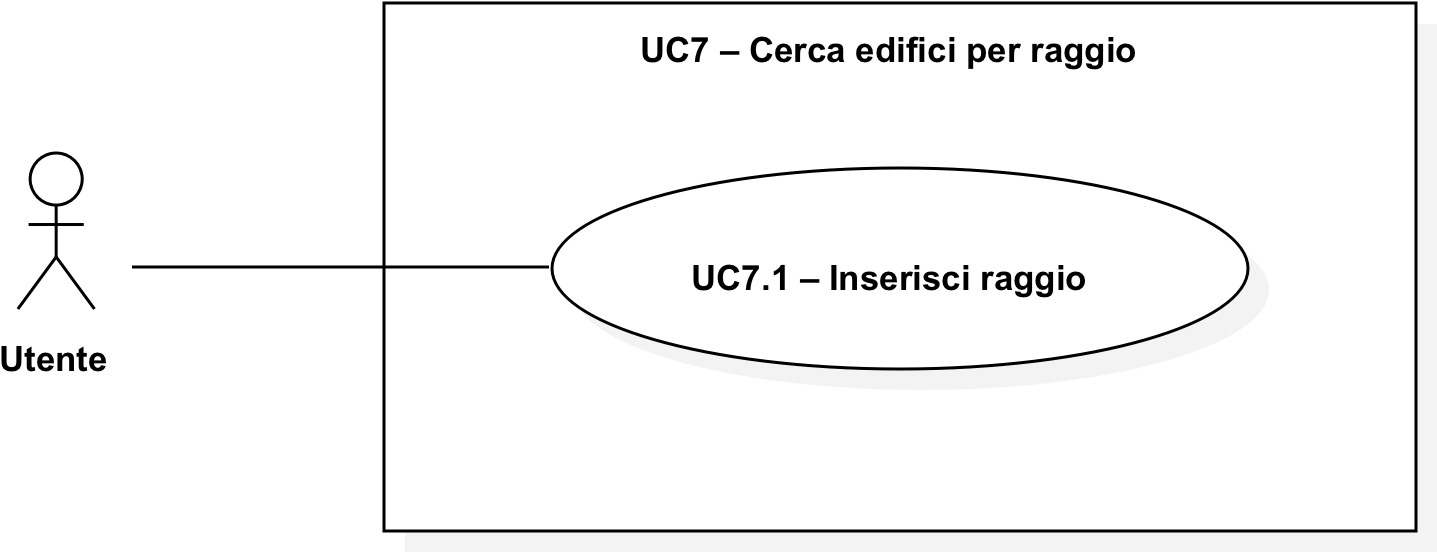
\includegraphics[scale=0.2]{img/UC7.png}
\caption{Caso d'uso UC7 - Cerca edifici per raggio}
 \end{figure}
\desc{l'utente cerca gli edifici abilitati entro un raggio.}\\\\
\pre{l'utente è alla ricerca degli edifici abilitati.}\\\\
\post{l'utente ha cercato gli edifici abilitati.}\\\\
\scen{l'utente cerca gli edifici abilitati entro un raggio tramite \UC{UC7.1}.
}\\\\
\att{Utente.}

\casoduso{UC7.1}{Inserisci raggio}
\desc{l'utente inserisce il raggio di ricerca degli edifici abilitati.}\\\\
\pre{l'utente è alla ricerca degli edifici abilitati.}\\\\
\post{l'utente ha inserito il raggio di ricerca degli edifici abilitati.}\\\\
\scen{l'utente inserisce il raggio di ricerca degli edifici abilitati.}\\\\
\att{Utente.}

\casoduso{UC9}{Visualizza lista edifici}
\desc{l'utente visualizza la lista degli edifici abilitati.}\\\\
\pre{l'utente ha cercato gli edifici.}\\\\
\post{l'utente ha visualizzato la lista degli edifici.}\\\\
\scen{l'utente visualizza la lista degli edifici abilitati.}\\\\
\att{Utente.}

\casoduso{UC10}{Visualizza edificio}
\begin{figure}[H]
\centering
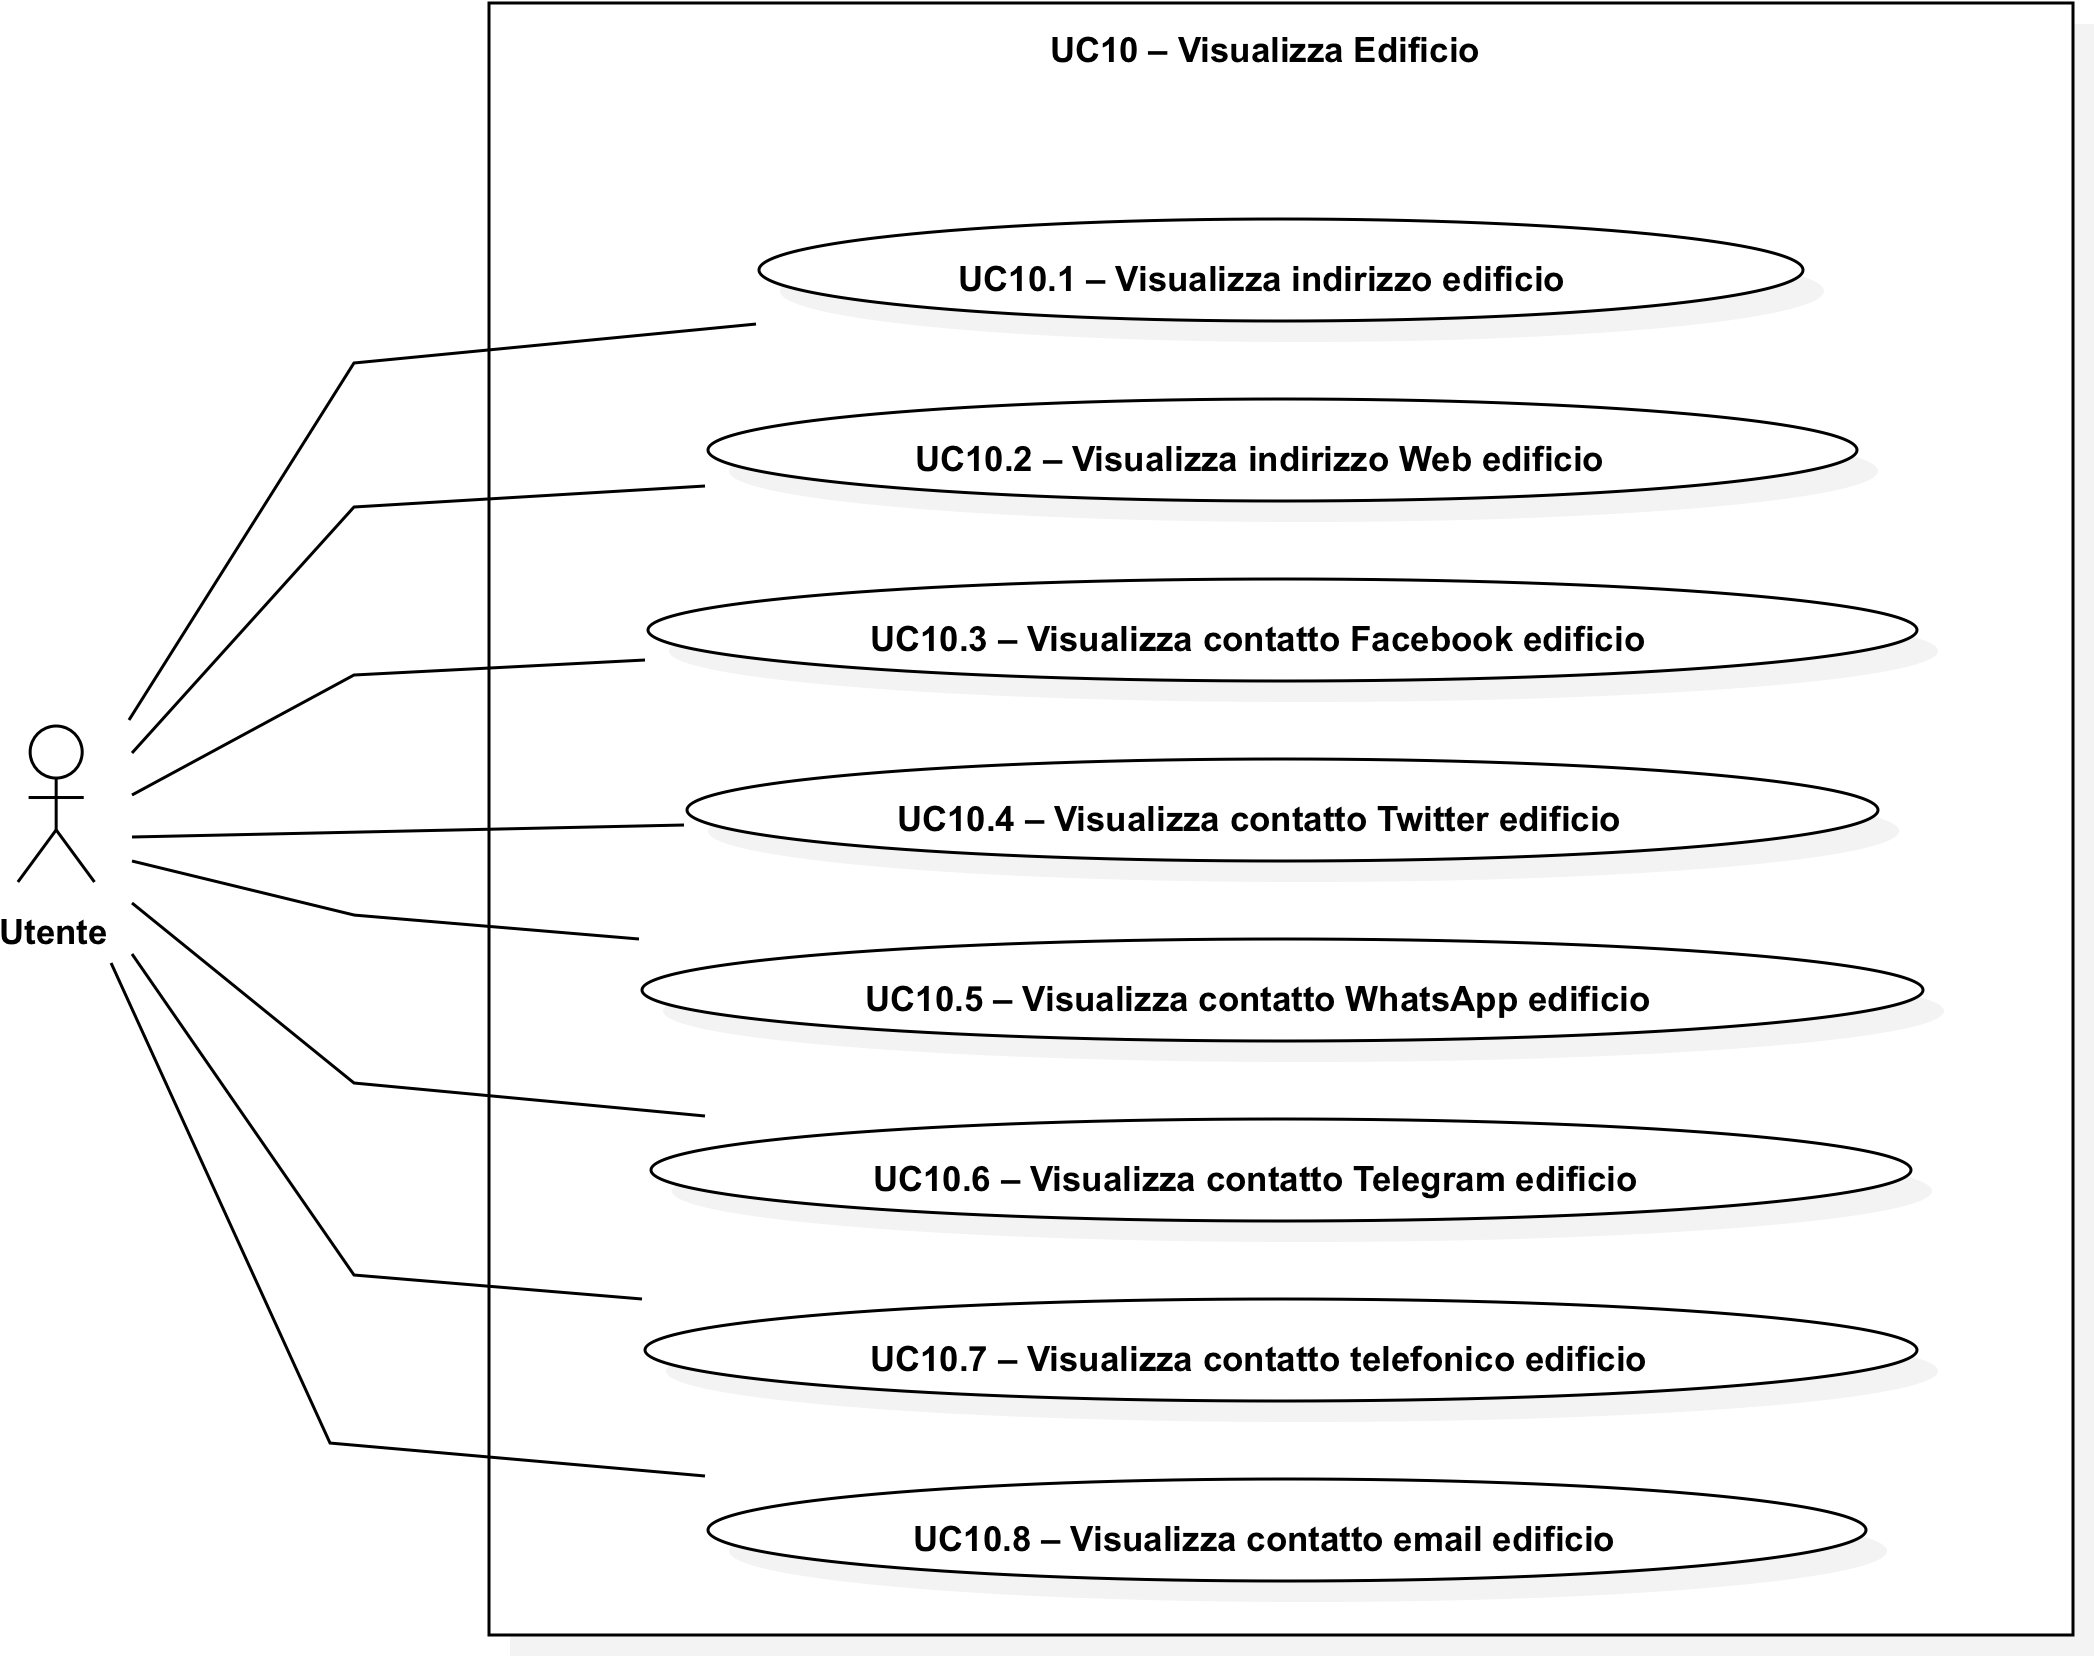
\includegraphics[scale=0.2]{img/UC10.png}
\caption{Caso d'uso UC10 - Visualizza edificio}
 \end{figure}
\desc{l'utente visualizza i dettagli di un edificio abilitato.}\\\\
\pre{l'utente ha visualizzato la lista degli edifici abilitati.}\\\\
\post{l'utente ha visualizzato i dettagli di un edificio abilitato.}\\\\
\scen{l'utente visualizza i dettagli di un edificio abilitato. In particolare visualizza:
\begin{itemize}
\item l'indirizzo (\UC{UC10.1});
\item l'indirizzo web dell' edificio (\UC{UC10.2});
\item i seguenti contatti:
\begin{itemize}
\item Facebook (\UC{UC10.3});
\item Twitter (\UC{UC10.4});
\item WhatsApp (\UC{UC10.5});
\item Telegram (\UC{UC10.6});
\item contatto telefonico (\UC{UC10.7});
\item email (\UC{UC10.8}).
\end{itemize}
\end{itemize}}\\\\
\att{Utente.}

\casoduso{UC10.1}{Visualizza indirizzo edificio}
\desc{l'utente visualizza l'indirizzo dell'edificio.}\\\\
\pre{l'utente richiede informazioni sull'edificio.}\\\\
\post{l'utente ha visualizzato l'indirizzo dell'edificio.}\\\\
\scen{l'utente visualizza l'indirizzo dell'edificio.}\\\\
\att{Utente.}

\casoduso{UC10.2}{Visualizza indirizzo web edificio}
\desc{l'utente visualizza l'indirizzo web dell'edificio.}\\\\
\pre{l'utente richiede informazioni sull'edificio.}\\\\
\post{l'utente ha visualizzato l'indirizzo web dell'edificio.}\\\\
\scen{l'utente visualizza l'indirizzo web dell'edificio.}\\\\
\att{Utente.}

\casoduso{UC10.3}{Visualizza contatto Facebook edificio}
\desc{l'utente visualizza il contatto Facebook dell'edificio.}\\\\
\pre{l'utente richiede informazioni per contattare l'edificio.}\\\\
\post{l'utente ha visualizzato il contatto Facebook dell'edificio.}\\\\
\scen{l'utente visualizza il contatto Facebook dell'edificio.}\\\\
\att{Utente.}

\casoduso{UC10.4}{Visualizza contatto Twitter edificio}
\desc{l'utente visualizza il contatto Twitter dell'edificio.}\\\\
\pre{l'utente richiede informazioni per contattare l'edificio.}\\\\
\post{l'utente ha visualizzato il contatto Twitter dell'edificio.}\\\\
\scen{l'utente visualizza il contatto Twitter dell'edificio.}\\\\
\att{Utente.}

\casoduso{UC10.5}{Visualizza contatto WhatsApp edificio}
\desc{l'utente visualizza il contatto WhatsApp dell'edificio.}\\\\
\pre{l'utente richiede informazioni per contattare l'edificio.}\\\\
\post{l'utente ha visualizzato il contatto WhatsApp dell'edificio.}\\\\
\scen{l'utente visualizza il contatto WhatsApp dell'edificio.}\\\\
\att{Utente.}

\casoduso{UC10.6}{Visualizza contatto Telegram edificio}
\desc{l'utente visualizza il contatto Telegram dell'edificio.}\\\\
\pre{l'utente richiede informazioni per contattare l'edificio.}\\\\
\post{l'utente ha visualizzato il contatto Telegram dell'edificio.}\\\\
\scen{l'utente visualizza il contatto Telegram dell'edificio.}\\\\
\att{Utente.}

\casoduso{UC10.7}{Visualizza contatto telefonico ufficio}
\desc{l'utente visualizza il contatto telefonico dell'edificio.}\\\\
\pre{l'utente richiede informazioni per contattare l'edificio.}\\\\
\post{l'utente ha visualizzato il contatto telefonico dell'edificio.}\\\\
\scen{l'utente visualizza il contatto telefonico dell'edificio.}\\\\
\att{Utente.}

\casoduso{UC10.8}{Visualizza email edificio}
\desc{l'utente visualizza l'email per contattare  l'edificio.}\\\\
\pre{l'utente richiede informazioni per contattare l'edificio.}\\\\
\post{l'utente ha visualizzato l'email per contattare  l'edificio.}\\\\
\scen{l'utente visualizza l'email per contattare  l'edificio.}\\\\
\att{Utente.}

\casoduso{UC11}{Registrazione}
\begin{figure}[H]
\centering
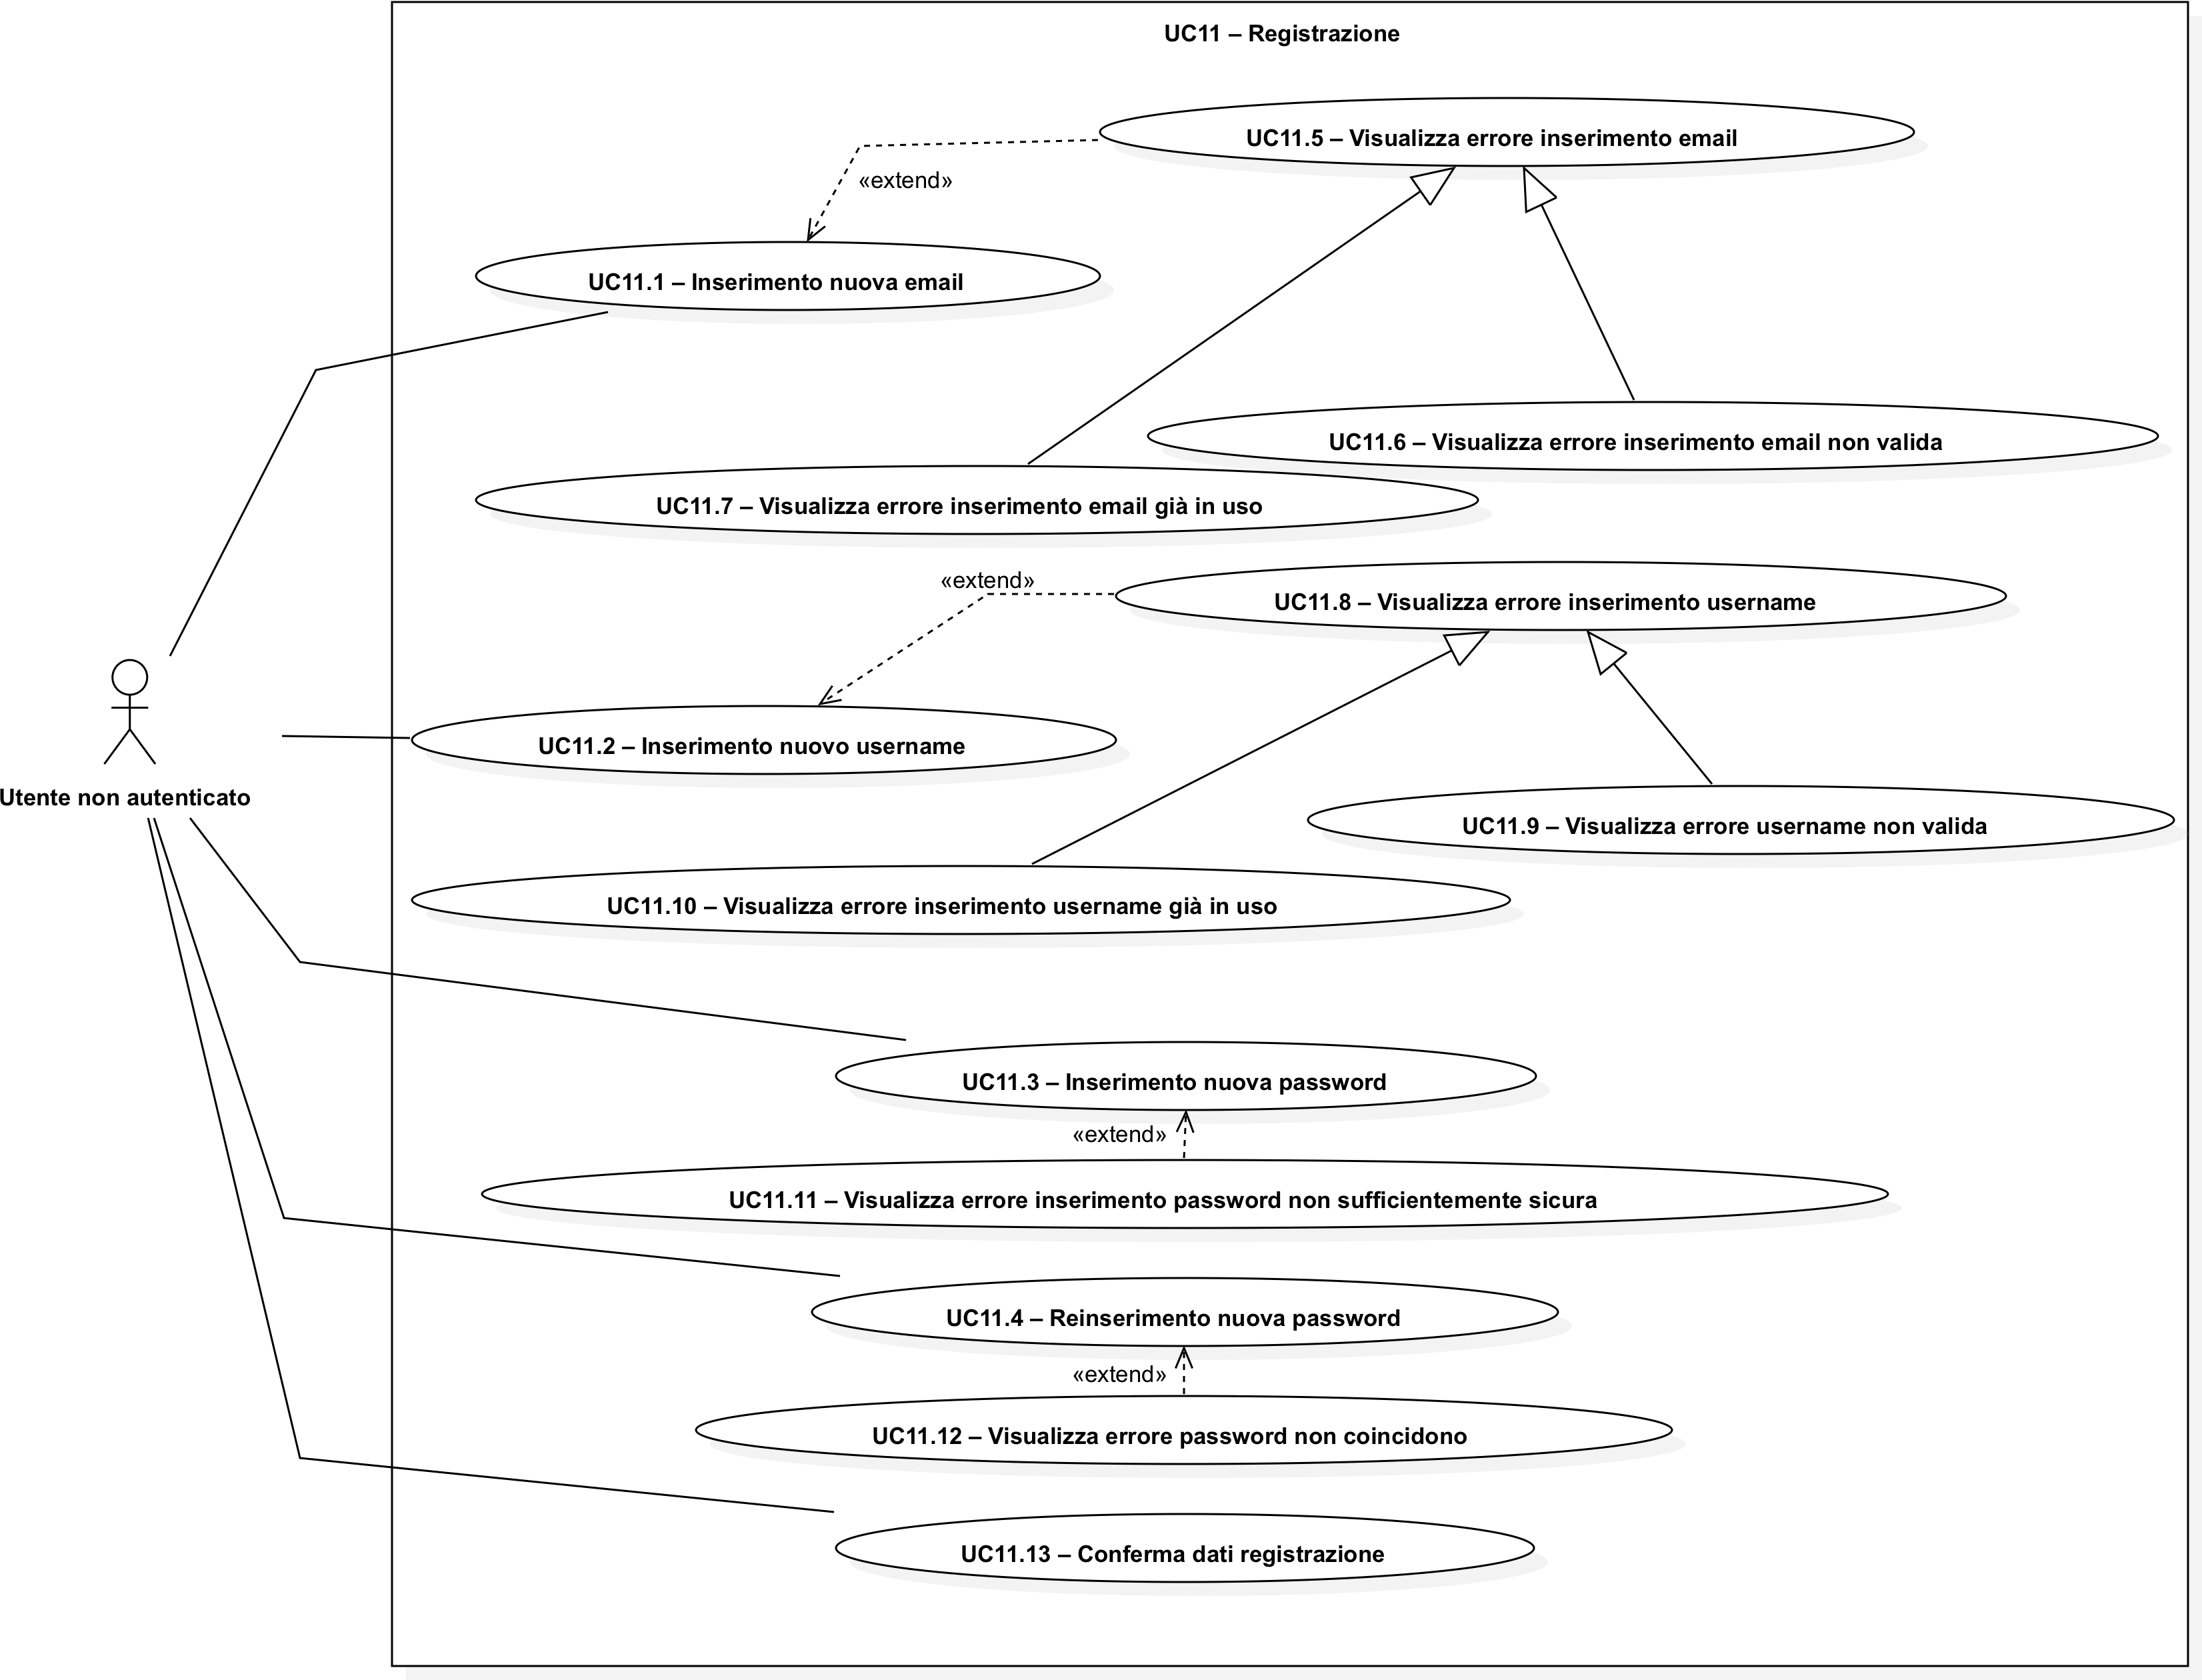
\includegraphics[scale=0.14]{img/UC11.png}
\caption{Caso d'uso UC11 - Registrazione}
 \end{figure}
\desc{l'utente si registra nel database inserendo un'email valida e una password sufficientemente sicura.}\\\\
\pre{l'utente non è registrato.}\\\\
\post{l'utente è registrato nel database.}\\\\
\scen{\begin{itemize}
\item \UC{UC11.1} l'utente inserisce un indirizzo email valido;
\item \UC{UC11.2} l'utente inserisce un username univoco;
\item \UC{UC11.3} l'utente inserisce una password sufficientemente sicura;
\item \UC{UC11.4} l'utente reinserisce la password precedentemente scelta;
\item \UC{UC11.13} l'utente conferma i dati inseriti.
\end{itemize}}\\\\
\att{Utente non autenticato.}

\casoduso{UC11.1}{Inserimento nuova email}
\desc{l'utente inserisce l'indirizzo email con cui desidera registrarsi.}\\\\
\pre{la connessione ad internet è attiva e l'App fornisce la pagina di registrazione.}\\\\
\post{l'utente ha inserito la email.}\\\\
\scen{l'utente inserisce il proprio indirizzo email per registrarsi.}\\\\
\scensec{ESTENSIONE \begin{itemize}
\item \UC{UC11.5} l'email inserita non è valida e viene visualizzato l'errore.
\end{itemize}}\\\\
\att{Utente non autenticato.}


\casoduso{UC11.2}{Inserimento nuovo username}
\desc{l'utente inserisce l'username con cui desidera registrarsi.}\\\\
\pre{la connessione ad internet è attiva e l'App fornisce la pagina di registrazione.}\\\\
\post{l'utente ha inserito l'username.}\\\\
\scen{l'utente inserisce l'username con cui desidera registrarsi.}\\\\
\scensec{ESTENSIONE \begin{itemize}
\item \UC{UC11.6} l'username inserito è già in uso e viene visualizzato l'errore.
\end{itemize}}\\\\
\att{Utente non autenticato.}

\casoduso{UC11.3}{Inserimento nuova password}
\desc{l'utente inserisce la password con cui desidera registrarsi.}\\\\
\pre{la connessione ad internet è attiva e l'App fornisce la pagina di registrazione.}\\\\
\post{l'utente ha inserito la password.}\\\\
\scen{l'utente inserisce la password con cui desidera registrarsi.}\\\\
\scensec{ESTENSIONE \begin{itemize}
\item \UC{UC11.11} la password inserita non è sufficientemente sicura e viene visualizzato l'errore.
\end{itemize}}\\\\
\att{Utente non autenticato.}

\casoduso{UC11.4}{Reinserimento nuova password}
\desc{l'utente reinserisce la nuova password.}\\\\
\pre{l'utente si trova nella pagina di registrazione.}\\\\
\post{l'utente ha reniserito la nuova password.}\\\\
\scen{l'utente reinserisce la nuova password.}\\\\
\scensec{ESTENSIONE \begin{itemize}
\item \UC{UC11.12}: la password reinserita non coincide con la nuova password e viene visualizzato l'errore.
\end{itemize}}\\\\
\att{Utente non autenticato.}

\casoduso{UC11.5}{Visualizza errore inserimento email}
\desc{l'utente visualizza l'errore il quale segnala che l'email non rispetta i requisiti richiesti.}\\\\
\pre{l'utente ha inserito una email non rispetta i requisiti richiesti.}\\\\
\post{l'utente ha visualizzato l'errore il quale segnala che l'email non rispetta i requisiti richiesti.}\\\\
\scen{l'utente visualizza l'errore il quale segnala che l'email non rispetta i requisiti richiesti}\\\\
\att{Utente non autenticato.}

\casoduso{UC11.6}{Visualizza errore inserimento email non valida}
\desc{l'utente visualizza un messaggio d'errore perché ha inserito un'email  non valida che non soddisfa il \Req{R0F1.2.7.1.1}.}\\\\
\pre{l'utente ha inserito un'email non valida.}\\\\
\post{l'utente viene notificato di aver inserito un'email non valida.}\\\\
\scen{l'utente visualizza un messaggio d'errore perché ha inserito un'email  non valida che non soddisfa il \Req{R0F1.2.7.1.1}.}\\\\
\att{Utente non autenticato.}

\casoduso{UC11.7}{Visualizza errore inserimento email già in uso}
\desc{l'utente viene notificato di aver inserito un'email già presente nel sistema.}\\\\
\pre{l'utente ha inserito un'email già presente nel sistema.}\\\\
\post{l'utente è stato notificato di aver inserito un'email già presente nel sistema.}\\\\
\scen{l'utente viene notificato di aver inserito un'email già presente nel sistema.}\\\\
\att{Utente non autenticato.}

\casoduso{UC11.8}{Visualizza errore inserimento username}
\desc{l'utente visualizza l'errore sull'inserimento dell'username.}\\\\
\pre{l'utente ha inserito un nuovo username che non soddisfa i requisiti richiesti.}\\\\
\post{l'utente ha visualizzato il messaggio di errore sull'inserimento dell'username.}\\\\
\scen{l'utente visualizza l'errore sull'inserimento dell'username.}\\\\
\att{Utente non autenticato.}

\casoduso{UC11.9}{Visualizza errore inserimento username non valido}
\desc{l'utente ha inserito un username che non rispetta il requisito \Req{R0F1.2.7.2.1}.}\\\\
\pre{l'utente ha inserito un username non valido.}\\\\
\post{l'utente viene notificato di aver inserito un username non valido.}\\\\
\scen{l'utente ha inserito un username che non rispetta il requisito \Req{R0F1.2.7.2.1}.}\\\\
\att{Utente non autenticato.}

\casoduso{UC11.10}{Visualizza errore inserimento username già in uso}
\desc{l'utente viene informato di aver inserito un username già in uso nel sistema.}\\\\
\pre{l'utente ha inserito un username già in uso nel sistema.}\\\\
\post{l'utente è stato informato di aver inserito un username già in uso nel sistema.}\\\\
\scen{l'utente viene informato di aver inserito un username già in uso nel sistema.}\\\\
\att{Utente non autenticato.}

\casoduso{UC11.11}{Visualizza errore password non sufficientemente sicura}
\desc{l'utente visualizza l'errore il quale segnala che la nuova password inserita non è sufficientemente sicura.}\\\\
\pre{l'utente ha inserito una nuova password non sufficientemente sicura.}\\\\
\post{l'utente ha visualizzato l'errore il quale segnala che la nuova password inserita non è sufficientemente sicura.}\\\\
\scen{l'utente visualizza l'errore il quale segnala che la nuova password inserita non è sufficientemente sicura.}\\\\
\att{Utente non autenticato.}

\casoduso{UC11.12}{Visualizza errore password reinserita non coincidente con la nuova password}
\desc{l'utente visualizza l'errore il quale segnala che la password reinserita non coincide con la nuova password.}\\\\
\pre{l'utente ha reinserito la password che non coincide con quella nuova precedentemente inserita.}\\\\
\post{l'utente ha visualizzato l'errore il quale segnala che la password reinserita non coincide con la nuova password.}\\\\
\scen{l'utente visualizza l'errore il quale segnala che la password reinserita non coincide con la nuova password.}\\\\
\att{Utente non autenticato.}

\casoduso{UC11.13}{Conferma dati registrazione}
\desc{l'utente conferma i dati di registrazione inseriti.}\\\\
\pre{l'utente ha inserito i dati per la registrazione.}\\\\
\post{l'utente ha confermato i dati inseriti per la registrazione.}\\\\
\scen{l'utente conferma i dati di registrazione inseriti.}\\\\
\att{Utente non autenticato.}

\casoduso{UC12}{Visualizza avviso di attivazione GPS}
\desc{l'utente visualizza il messaggio di invito all'attivazione del GPS.}\\\\
\pre{il GPS non è attivo sul dispositivo dell'utente.}\\\\
\post{l'utente ha visualizzato il messaggio di invito all'attivazione del GPS.}\\\\
\scen{l'utente visualizza il messaggio di invito all'attivazione del GPS.}\\\\
\att{Utente.}

\casoduso{UC13}{Visualizza avviso di attivazione della connessione ad internet}
\desc{l'utente visualizza il messaggio di invito all'attivazione della connessione ad internet.}\\\\
\pre{la connessione ad internet non è attiva sul dispositivo dell'utente.}\\\\
\post{l'utente ha visualizzato il messaggio di invito all'attivazione della connessione ad internet.}\\\\
\scen{l'utente visualizza il messaggio di invito all'attivazione della connessione ad internet.}\\\\
\att{Utente.}

\casoduso{UC14}{Errore autenticazione}
\desc{L'utente visualizza l'errore di autenticazione nel quale viene specificato che non ha inserito i dati corretti.}\\\\
\pre{l'utente ha inserito i dati di autenticazione.}\\\\
\post{l'utente ha visualizzato l'errore di autenticazione.}\\\\
\scen{L'utente visualizza l'errore di autenticazione nel quale viene specificato che non ha inserito i dati corretti.}\\\\
\att{Utente non autenticato.}

\casoduso{UC15}{Visualizza lista percorsi salvati}
\desc{l'utente visualizza la lista dei percorsi salvati.}\\\\
\pre{l'utente ha l'app installata e in esecuzione.}\\\\
\post{l'utente ha visualizzato i percorsi salvati.}\\\\
\scen{l'utente visualizza la lista dei percorsi salvati.}\\\\
\scensec{ESTENSIONE: \begin{itemize}
\item \UC{UC16} l'utente non è autenticato e visualizza l'invito ad autenticarsi per visualizzare la lista dei percorsi salvati;
\item \UC{UC17} l'utente visualizza l'invito a registrarsi per poi autenticarsi e visualizzare la lista dei percorsi salvati;
\item \UC{UC18} l'utente non ha alcun percorso salvato e visualizza l'invito a svolgerene almeno uno.
\end{itemize}}\\\\
\att{Utente.}

\casoduso{UC16}{Visualizza invito ad autenticarsi}
\desc{l'utente visualizza l'invito ad autenticarsi.}\\\\
\pre{l'utente non è autenticato.}\\\\
\post{l'utente ha visualizzato l'invito ad autenticarsi.}\\\\
\scen{l'utente visualizza l'invito ad autenticarsi.}\\\\
\att{Utente non autenticato.}

\casoduso{UC17}{Visualizza invito a registrarsi}
\desc{l'utente visualizza l'invito a registrarsi.}\\\\
\pre{l'utente non è registrato nel database dell'app.}\\\\
\post{l'utente ha visualizzato l'invito a registrarsi.}\\\\
\scen{l'utente visualizza l'invito a registrarsi.}\\\\
\att{Utente non autenticato.}

\casoduso{UC18}{Visualizza invito a svolgere un percorso}
\desc{l'utente visualizza l'invito a svolgere almeno un percorso.}\\\\
\pre{l'utente non ha svolto nessun percorso.}\\\\
\post{l'utente ha visualizzato l'invito a svolgere almeno un percorso.}\\\\
\scen{l'utente visualizza l'invito a svolgere almeno un percorso.}\\\\
\att{Utente.}

\casoduso{UC19}{Visualizza dettagli percorso salvato}
\desc{l'utente visualizza i dettagli di un percorso salvato.}\\\\
\pre{l'utente ha salvato almeno un percorso.}\\\\
\post{l'utente ha visualizzato i dettagli di un percorso salvato.}\\\\
\scen{l'utente visualizza i dettagli di un percorso salvato.}\\\\
\att{Utente autenticato.}

\casoduso{UC20}{Recupero credenziali}
\begin{figure}[H]
\centering
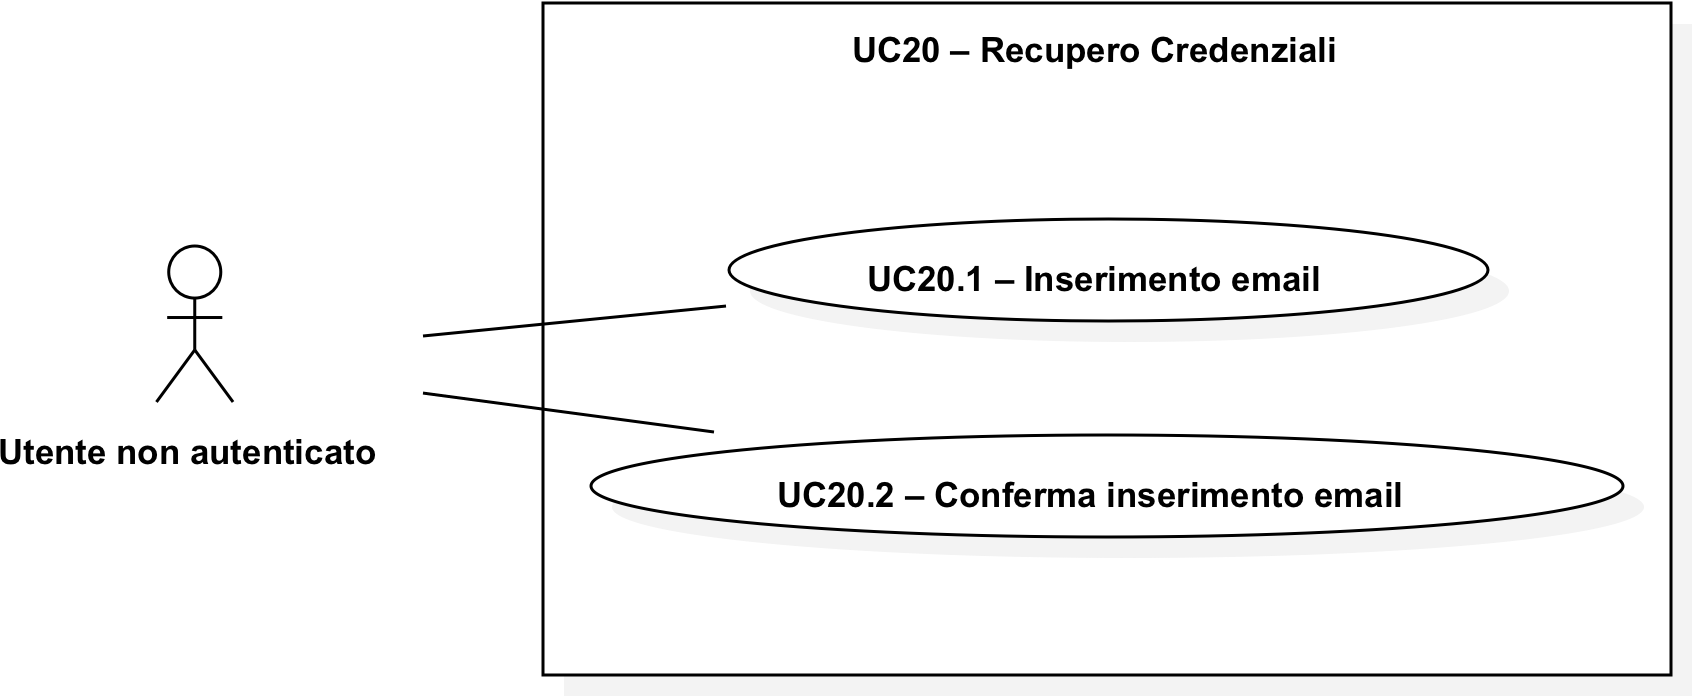
\includegraphics[scale=0.2]{img/UC20.png}
\caption{Caso d'uso UC20 - Recupero credenziali}
 \end{figure}
\desc{l'utente richiede le credenziali d'accesso.}\\\\
\pre{l'utente non ricorda le credenziali per accedere al suo profilo.}\\\\
\post{l'utente ha richiesto le proprie credenziali di acesso.}\\\\
\scen{l'utente richiede le credenziali d'accesso:
\begin{itemize}
\item \UC{UC20.1} l'utente inserisce l'email con cui è registrato
\item \UC{UC20.2} l'utente conferma l'email inserita.
\end{itemize}}\\\\
\att{Utente non autenticato.}

\casoduso{UC20.1}{Inserimento email}
\desc{l'utente inserisce l'email con cui si era registrato.}\\\\
\pre{l'utente non riesce ad effettuare il login perché non è in possesso delle credenziali.}\\\\
\post{l'utente ha inserito l'email con cui si era registrato.}\\\\
\scen{l'utente inserisce l'email con cui si era registrato.}\\\\
\att{Utente non autenticato.}

\casoduso{UC20.2}{Conferma inserimento email}
\desc{l'utente conferma l'email che ha inserito per il recupero delle credenziali.}\\\\
\pre{l'utente ha inserito l'email per il recupero delle credenziali.}\\\\
\post{l'utente ha confermato l'inserimento della mail per il recupero delle credenziali.}\\\\
\scen{l'utente conferma l'email che ha inserito per il recupero delle credenziali.}\\\\
\att{Utente non autenticato.}

\casoduso{UC21}{Visualizza percorsi disponibili}
\desc{l'utente visualizza i percorsi disponibili nell'edificio in cui si trova.}\\\\
\pre{l'utente ha attivato i servizi di localizzazione, bluetooth e la connessione ad Internet; l'utente è in un edificio abilitato; l'utente è in prossimità di un beacon.}\\\\
\post{l'utente ha visualizzato la lista dei percorsi disponibili.}\\\\
\scen{l'utente visualizza i percorsi disponibili nell'edificio in cui si trova.}\\\\
\att{Utente.}

\casoduso{UC22}{Visualizza lista dei percorsi percorsi}
\desc{l'utente visualizza la lista dei percorsi presenti nell'edificio.}\\\\
\pre{l'utente ha i servizi di localizzazione, bluetooth e connessione a Internet attivi.}\\\\
\post{l'utente ha visualizzato i percorsi presenti nell'edificio.}\\\\
\scen{l'utente visualizza la lista dei percorsi presenti nell'edificio.}\\\\
\att{Utente.}

\casoduso{UC23}{Visualizza percorso}
\desc{l'utente visualizza i dettagli di un percorso.}\\\\
\pre{l'utente ha visualizzato la lista degli edifici.}\\\\
\post{l'utente ha visualizzato i dettagli di un percorso.}\\\\
\scen{l'utente visualizza i dettagli di un percorso e se si trova nell'edificio del percorso può:
\begin{itemize}
\item \UC{UC3} iniziare a svolgere il percorso.
\end{itemize}}\\\\
\att{Utente.}


\newpage
\section{Requisiti}
\label{sec:Requisiti}
Di seguito verranno elencati i requisiti individuati grazie all'analisi del \gl{capitolato}, la produzione dei casi d'uso, dagli incontri con il Proponente o a necessità interne. Verranno catalogati in tabelle contenenti il codice del requisito, la tipologia, la descrizione e la fonte.\\
I codici dei requisiti seguiranno la forma:
\begin{center}
	R[importanza][tipo][identificativo]
\end{center}
\begin{itemize}
	\item \textbf{Importanza}:indica se il requisito è:
	\begin{enumerate}
		\item \textbf{0}: obbligatorio;
		\item \textbf{1}: desiderabile;
		\item \textbf{2}: opzionale.
	\end{enumerate}
	\item \textbf{Tipo}: indica se è di tipo:
	\begin{enumerate}
		\item \textbf{F}: funzionale;
		\item \textbf{Q}: di qualità;
		\item \textbf{P}: prestazionale;
		\item \textbf{V}: di vincolo.
	\end{enumerate}
	\item \textbf{Identificativo}: è il codice univoco e gerarchico che automaticamente il \gl{software} assegna al requisito (esempio: 4.2.1).
\end{itemize}

\label{sec:Requisiti}
\begin{tabella}{!{\VRule}c!{\VRule}c!{\VRule}X[1,m,c]!{\VRule}c!{\VRule}}\intestazionefourcol{Requisito}{Tipologia}{Descrizione}{Fonti}\requisito{R0V1} & \cellacaporiga{Vincolo \\ Obbligatorio } & Il prodotto deve sfruttare la tecnologia dei beacon per poter eseguire le sue funzionalità principali. & \cellacaporiga{Capitolato } \\ 
\requisito{R0V1.1} & \cellacaporiga{Vincolo \\ Obbligatorio } & Il prodotto deve usare la tecnologia dei beacon per segnare le tappe dei percorsi. & \cellacaporiga{Verbale 2016-03-21 } \\ 
\requisito{R0V2} & \cellacaporiga{Vincolo \\ Obbligatorio } & L'app deve funzionare su dispositivi mobile. & \cellacaporiga{Capitolato } \\ 
\requisito{R0V2.1} & \cellacaporiga{Vincolo \\ Obbligatorio } & L'applicativo verrà sviluppato per dispositivi Android con almeno la versione 5.0. & \cellacaporiga{Interno } \\ 
\requisito{R2V2.2} & \cellacaporiga{Vincolo \\ Opzionale } & L'applicativo verrà sviluppato per dispositivi iOS con almeno la versione 9.0. & \cellacaporiga{Interno } \\ 
\hiderowcolors
\caption{Tracciamento requisiti di vincolo}
\end{tabella}

\newpage
\subsection{Requisiti Funzionali}
\label{sub:Requisiti Funzionali}
\begin{tabella}{!{\VRule}c!{\VRule}c!{\VRule}X[1,m,c]!{\VRule}c!{\VRule}}\intestazionefourcol{Requisito}{Tipologia}{Descrizione}{Fonti}\requisito{R0F1} & \cellacaporiga{Funzionale \\ Obbligatorio } & L'utente deve poter possedere un account registrato nel database. & \cellacaporiga{\UC{UC1.1} } \\
\requisito{R0F1.1} & \cellacaporiga{Funzionale \\ Obbligatorio } & Il sistema deve permettere all'utente di autenticarsi. & \cellacaporiga{\UC{UC1.1.1} } \\
\requisito{R0F1.1.1} & \cellacaporiga{Funzionale \\ Obbligatorio } & Il sistema deve chiedere all'utente l'email per la procedura di autenticazione. & \cellacaporiga{\UC{UC1.1.1.1} } \\
\requisito{R0F1.1.2} & \cellacaporiga{Funzionale \\ Obbligatorio } & Il sistema deve chiedere all'utente la password per la procedura di autenticazione. & \cellacaporiga{\UC{UC1.1.1.2} } \\
\requisito{R0F1.1.3} & \cellacaporiga{Funzionale \\ Obbligatorio } & Il sistema deve permettere all'utente di confermare i dati inseriti per la procedura di autenticazione. & \cellacaporiga{\UC{UC1.1.1.3} } \\
\requisito{R0F1.1.4} & \cellacaporiga{Funzionale \\ Obbligatorio } & Se i dati confermati dall'utente sono validi egli viene autenticato. & \cellacaporiga{\UC{UC1.1.1.4} } \\
\requisito{R0F1.1.5} & \cellacaporiga{Funzionale \\ Obbligatorio } & Il sistema deve segnalare all'utente ogni eventuale errore durante la procedura di autenticazione. & \cellacaporiga{\UC{UC1.1.3} } \\
\requisito{R0F1.1.5.1} & \cellacaporiga{Funzionale \\ Obbligatorio } & Il sistema interrompe la procedura di autenticazione se l'email non corrisponde a nessuna di quelle registrate. & \cellacaporiga{Interno } \\
\requisito{R0F1.1.5.2} & \cellacaporiga{Funzionale \\ Obbligatorio } & Il sistema interrompe la procedura di autenticazione se la password non corrisponde a quella associata all'email. & \cellacaporiga{Interno } \\
\requisito{R0F1.1.5.3} & \cellacaporiga{Funzionale \\ Obbligatorio } & Il dispositivo informa l'utente dell'errore nell'inserimento dei dati. & \cellacaporiga{\UC{UC1.1.3.1} } \\
\requisito{R0F1.1.5.4} & \cellacaporiga{Funzionale \\ Obbligatorio } & L'utente può richiedere una nuova password inserendo l'email. & \cellacaporiga{\UC{UC1.1.3.2} } \\
\requisito{R0F1.1.5.4.1} & \cellacaporiga{Funzionale \\ Obbligatorio } & L'utente deve inserire l'email per proseguire. & \cellacaporiga{Interno } \\
\requisito{R0F1.1.5.4.2} & \cellacaporiga{Funzionale \\ Obbligatorio } & L'utente riceve un'email all'indirizzo inserito con una password casuale. & \cellacaporiga{\UC{UC1.1.3.2} } \\
\requisito{R0F1.1.5.4.3} & \cellacaporiga{Funzionale \\ Obbligatorio } & La password dell'utente viene sostituita con la password inviata. & \cellacaporiga{Interno } \\
\requisito{R0F1.2} & \cellacaporiga{Funzionale \\ Obbligatorio } & L'utente deve poter creare un proprio account per poter usufruire delle relative funzionalità. & \cellacaporiga{\UC{UC1.1.2} } \\
\requisito{R0F1.2.1} & \cellacaporiga{Funzionale \\ Obbligatorio } & La registrazione chiede l'email all'utente. & \cellacaporiga{\UC{UC1.1.2.1} } \\
\requisito{R0F1.2.2} & \cellacaporiga{Funzionale \\ Obbligatorio } & La registrazione chiede lo username all'utente. & \cellacaporiga{\UC{UC1.1.2.2} } \\
\requisito{R0F1.2.3} & \cellacaporiga{Funzionale \\ Obbligatorio } & La registrazione chiede la password all'utente. & \cellacaporiga{\UC{UC1.1.2.3} } \\
\requisito{R0F1.2.4} & \cellacaporiga{Funzionale \\ Obbligatorio } & Il sistema chiede all'utente di confermare i dati della propria registrazione. & \cellacaporiga{\UC{UC1.1.2.4} } \\
\requisito{R0F1.2.5} & \cellacaporiga{Funzionale \\ Obbligatorio } & Se i dati confermati dall'utente sono validi il suo account viene registrato. & \cellacaporiga{Interno } \\
\requisito{R0F1.2.5.1} & \cellacaporiga{Funzionale \\ Obbligatorio } & L'utente viene automaticamente autenticato. & \cellacaporiga{Interno } \\
\requisito{R0F1.2.6} & \cellacaporiga{Funzionale \\ Obbligatorio } &  	Il sistema deve segnalare all'utente gli eventuali problemi di registrazione. & \cellacaporiga{\UC{UC1.1.4} } \\
\requisito{R0F1.2.6.1} & \cellacaporiga{Funzionale \\ Obbligatorio } &  	L'email deve avere un formato valido. Deve contenere una '@' preceduto da altri caratteri seguito da un dominio valido. & \cellacaporiga{Interno } \\
\requisito{R0F1.2.6.2} & \cellacaporiga{Funzionale \\ Obbligatorio } & L'email non dev'essere già in uso da un altro utente. & \cellacaporiga{Interno } \\
\requisito{R0F1.2.6.3} & \cellacaporiga{Funzionale \\ Obbligatorio } & Lo username non deve essere già in uso da un altro utente. & \cellacaporiga{Interno } \\
\requisito{R0F1.2.6.4} & \cellacaporiga{Funzionale \\ Obbligatorio } & La password deve contenere un minimo di 6 caratteri e un massimo di 16. & \cellacaporiga{Interno } \\
\requisito{R0F2} & \cellacaporiga{Funzionale \\ Obbligatorio } & L'utente deve poter fare il logout. & \cellacaporiga{\UC{UC1.2} } \\
\requisito{R0F3} & \cellacaporiga{Funzionale \\ Obbligatorio } & L'utente deve poter scegliere quale percorso fare tra quelli disponibili nel luogo dove si trova. & \cellacaporiga{\UC{UC1.3} } \\
\requisito{R0F3.1} & \cellacaporiga{Funzionale \\ Obbligatorio } & L'utente gioca il percorso selezionato fino alla sua conclusione. & \cellacaporiga{\UC{UC1.3.1} } \\
\requisito{R0F3.1.1} & \cellacaporiga{Funzionale \\ Obbligatorio } & L'utente cerca il \gl{beacon} corrispondente alla prima stazione. & \cellacaporiga{\UC{UC1.3.1.1} } \\
\requisito{R0F3.1.1.1} & \cellacaporiga{Funzionale \\ Obbligatorio } & Se il dispositivo dell'utente trova il \gl{beacon} corrispondente alla stazione corretta l'utente può cominciare a giocare.  & \cellacaporiga{Interno } \\
\requisito{R0F3.1.1.2} & \cellacaporiga{Funzionale \\ Obbligatorio } & I \gl{beacon} che il dispositivo rileva non inerenti con la stazione cercata devono essere ignorati dall'app. & \cellacaporiga{Interno } \\
\requisito{R1F3.1.1.3} & \cellacaporiga{Funzionale \\ Desiderabile } & L'utente può chiedere aiuto se non riesce a trovare la prima stazione o se pensa che il dispositivo non riesca a rilevare il \gl{beacon} corretto. & \cellacaporiga{Interno } \\
\requisito{R2F3.1.1.4} & \cellacaporiga{Funzionale \\ Opzionale } & Il dispositivo può sfruttare dei \gl{beacon} aggiuntivi ed estranei al percorso per segnalare all'utente la distanza tra lui e la stazione. & \cellacaporiga{Interno } \\
\requisito{R2F3.1.1.4.1} & \cellacaporiga{Funzionale \\ Opzionale } & La distanza viene espressa con dei valori approssimativi (ad esempio delle tacche) per aiutare l'utente a capire se si sta allontanando o avvicinando alla stazione e quanto è distante approssimativamente. & \cellacaporiga{Interno } \\
\requisito{R0F3.1.2} & \cellacaporiga{Funzionale \\ Obbligatorio } & L'utente gioca la prova relativa a quella stazione. & \cellacaporiga{\UC{UC1.3.1.2} } \\
\requisito{R0F3.1.2.1} & \cellacaporiga{Funzionale \\ Obbligatorio } & La prova proposta all'utente è una fra quelle disponibili. & \cellacaporiga{Interno } \\
\requisito{R0F3.1.2.2} & \cellacaporiga{Funzionale \\ Obbligatorio } & L'app mostra le istruzioni della prova. & \cellacaporiga{\UC{UC1.3.1.2.1} } \\
\requisito{R0F3.1.2.3} & \cellacaporiga{Funzionale \\ Obbligatorio } & L'utente deve poter svolgere la prova. & \cellacaporiga{\UC{UC1.3.1.2.2} } \\
\requisito{R0F3.1.2.4} & \cellacaporiga{Funzionale \\ Obbligatorio } & Finita la prova il dispositivo deve mostrare il risultato ottenuto. & \cellacaporiga{\UC{UC1.3.1.2.3} } \\
\requisito{R0F3.1.2.5} & \cellacaporiga{Funzionale \\ Obbligatorio } & Finita la prova l'utente può proseguire il percorso o averlo terminato. & \cellacaporiga{Interno } \\
\requisito{R0F3.1.2.5.1} & \cellacaporiga{Funzionale \\ Obbligatorio } & Se la prova non è l'ultima l'app indica qual'è la prossima stazione. & \cellacaporiga{Interno } \\
\requisito{R0F3.1.2.5.1.1} & \cellacaporiga{Funzionale \\ Obbligatorio } & L'app mostra all'utente le informazioni per trovare la prossima stazione. & \cellacaporiga{Interno } \\
\requisito{R0F3.1.2.5.2} & \cellacaporiga{Funzionale \\ Obbligatorio } & Se la prova è l'ultima l'utente ha finito il percorso. & \cellacaporiga{Interno } \\
\requisito{R0F3.2} & \cellacaporiga{Funzionale \\ Obbligatorio } & Quando il percorso è finito il dispositivo mostra all'utente il riepilogo dei dati suoi e generali. & \cellacaporiga{\UC{UC1.3.2} } \\
\requisito{R0F3.2.1} & \cellacaporiga{Funzionale \\ Obbligatorio } & Il dispositivo mostra il tempo totale della prova. & \cellacaporiga{\UC{UC1.3.2.1} } \\
\requisito{R0F3.2.1.1} & \cellacaporiga{Funzionale \\ Obbligatorio } & La durata totale viene misurata da quando si accetta di cominciare il percorso fino a quando si conferma la soulzione dell'ultima prova. & \cellacaporiga{Interno } \\
\requisito{R0F3.2.2} & \cellacaporiga{Funzionale \\ Obbligatorio } & Il dispositivo mostra il tempo totale impiegato per eseguire le prove. & \cellacaporiga{\UC{UC1.3.2.2} } \\
\requisito{R0F3.2.2.1} & \cellacaporiga{Funzionale \\ Obbligatorio } & Il tempo totale per eseguire le prove viene calcolato sommando i tempi impiegati per eseguire ogni prova (in pratica è il tempo totale senza considerare gli spostamenti effettuati per cambiare stazione). & \cellacaporiga{Interno } \\
\requisito{R0F3.2.2.1.1} & \cellacaporiga{Funzionale \\ Obbligatorio } & La durata della prova viene misurata da quando si accetta di affrontarla fino alla conferma della soluzione (comprende solo il tempo dal termine dell'\UC{1.2.1} fino al termine dell\UC{1.2.2}). & \cellacaporiga{Interno } \\
\requisito{R0F3.2.3} & \cellacaporiga{Funzionale \\ Obbligatorio } & Il dispositivo mostra il punteggio totale ottenuto. & \cellacaporiga{\UC{UC1.3.2.3} } \\
\requisito{R0F3.2.3.1} & \cellacaporiga{Funzionale \\ Obbligatorio } & Il punteggio totale viene calcolato sommando il numero di punti ottenuto in ogni singola prova. & \cellacaporiga{Interno } \\
\requisito{R0F3.2.3.1.1} & \cellacaporiga{Funzionale \\ Obbligatorio } & Il punteggio di ogni singola prova viene calcolato in base al tipo di prova affrontata. & \cellacaporiga{Interno } \\
\requisito{R1F3.2.3.2} & \cellacaporiga{Funzionale \\ Desiderabile } & Il dispositivo informa l'utente se il risultato ottenuto è il suo nuovo record per quel percorso. & \cellacaporiga{Interno } \\
\requisito{R0F3.2.4} & \cellacaporiga{Funzionale \\ Obbligatorio } & Il dispositivo mostra la posizione che l'utente ha raggiunto con il punteggio ottenuto. & \cellacaporiga{\UC{UC1.3.2.4} } \\
\requisito{R0F3.2.4.1} & \cellacaporiga{Funzionale \\ Obbligatorio } & Se il numero totale di punteggi salvati da tutti gli utenti per quella prova è minore o uguale a 10 viene mostrata l'intera classifica. & \cellacaporiga{Interno } \\
\requisito{R0F3.2.4.2} & \cellacaporiga{Funzionale \\ Obbligatorio } & Se il numero totale di punteggi salvati da tutti gli utenti per quella prova è maggiore di 10 vengono mostrati in ordine i primi 3 risultati della classifica, i tre risultati subito sopra alla posizione dell'utente, il punteggio dell'utente e i 3 risultati subito sotto l'utente. & \cellacaporiga{Interno } \\
\requisito{R0F3.2.5} & \cellacaporiga{Funzionale \\ Obbligatorio } & Il dispositivo visualizza la prova con il maggior numero di punti realizzati. & \cellacaporiga{\UC{UC1.3.2.5} } \\
\requisito{R0F3.2.6} & \cellacaporiga{Funzionale \\ Obbligatorio } & Il dispositivo visualizza la prova con il minor numero di punti realizzati. & \cellacaporiga{\UC{UC1.3.2.6} } \\
\requisito{R0F3.3} & \cellacaporiga{Funzionale \\ Obbligatorio } & L'utente autenticato può salvare il risultato ottenuto. & \cellacaporiga{\UC{UC1.3.3} } \\
\requisito{R0F4} & \cellacaporiga{Funzionale \\ Obbligatorio } & L'utente deve poter visualizzare delle informazioni sull'app. & \cellacaporiga{\UC{UC1.4} } \\
\requisito{R0F4.1} & \cellacaporiga{Funzionale \\ Obbligatorio } & L'utente deve poter visualizzare una schermata con una descrizione generale dell'app. & \cellacaporiga{\UC{UC1.4.1} } \\
\requisito{R0F4.2} & \cellacaporiga{Funzionale \\ Obbligatorio } & L'utente deve poter accedere alla pagina web relativa all'app tramite un link presente all'interno dell'app. & \cellacaporiga{\UC{UC1.4.2} } \\
\requisito{R0F4.2.1} & \cellacaporiga{Funzionale \\ Obbligatorio } & Nella pagina web l'utente deve trovare una descrizione dettagliata dell'app. & \cellacaporiga{Interno } \\
\requisito{R0F4.3} & \cellacaporiga{Funzionale \\ Obbligatorio } & L'utente deve poter inviare una segnalazione in caso di errore. & \cellacaporiga{\UC{UC1.4.3} } \\
\requisito{R2F4.3.1} & \cellacaporiga{Funzionale \\ Opzionale } & Quando l'utente clicca il pulsante per inviare la segnalazione viene aperta una nuova email da scrivere tramite il gestore di email predefinito. Nell'email il destinatario viene impostato con l'email destinata alle segnalazioni. & \cellacaporiga{Interno } \\
\requisito{R2F4.3.2} & \cellacaporiga{Funzionale \\ Opzionale } & Quando l'utente clicca sul pulsante della segnalazione si apre una schermata dove l'utente seleziona delle caratteristiche per determinare l'errore avuto. & \cellacaporiga{Interno } \\
\requisito{R2F4.3.2.1} & \cellacaporiga{Funzionale \\ Opzionale } & L'utente seleziona il tipo di errore avuto. & \cellacaporiga{Interno } \\
\requisito{R2F4.3.2.2} & \cellacaporiga{Funzionale \\ Opzionale } & L'utente può selezionare l'eventuale stazione dove si è verificato l'errore. & \cellacaporiga{Interno } \\
\requisito{R2F4.3.2.3} & \cellacaporiga{Funzionale \\ Opzionale } & La conferma della schermata invia un'email all'indirizzo destinato alla segnalazione errori avente un testo predefinito a seconda dell'errore segnalato. & \cellacaporiga{Interno } \\
\requisito{R0F5} & \cellacaporiga{Funzionale \\ Obbligatorio } & L'utente autenticato deve poter visualizzare i risultati dei percorsi effettuati precedentemente. & \cellacaporiga{\UC{UC1.5} } \\
\requisito{R0F5.1} & \cellacaporiga{Funzionale \\ Obbligatorio } & Se l'utente è autenticato e ha dei percorsi salvati deve poterne visualizzare l'elenco. & \cellacaporiga{\UC{UC1.5.1} } \\
\requisito{R0F5.1.1} & \cellacaporiga{Funzionale \\ Obbligatorio } & Se l'utente clicca su un percorso il dispositivo deve visualizzare tutte le informazioni salvate. & \cellacaporiga{\UC{UC1.5.1.1} } \\
\requisito{R0F5.1.1.1} & \cellacaporiga{Funzionale \\ Obbligatorio } & Il dispositivo deve visualizzare il nome del percorso. & \cellacaporiga{Interno } \\
\requisito{R0F5.1.1.2} & \cellacaporiga{Funzionale \\ Obbligatorio } & Il dispositivo deve visualizzare il nome del luogo dove si è svolto il percorso. & \cellacaporiga{Interno } \\
\requisito{R0F5.1.1.3} & \cellacaporiga{Funzionale \\ Obbligatorio } & Il dispositivo deve visualizzare la data in cui si è svolto il percorso. & \cellacaporiga{Interno } \\
\requisito{R0F5.1.1.4} & \cellacaporiga{Funzionale \\ Obbligatorio } & Il dispositivo deve visualizzare il risultato del percorso. & \cellacaporiga{Interno } \\
\requisito{R0F5.1.1.5} & \cellacaporiga{Funzionale \\ Obbligatorio } & Il dispositivo deve visualizzare l'ora di inizio del percorso. & \cellacaporiga{Interno } \\
\requisito{R0F5.1.1.6} & \cellacaporiga{Funzionale \\ Obbligatorio } & Il dispositivo deve visualizzare l'ora di fine del percorso. & \cellacaporiga{Interno } \\
\requisito{R2F5.1.1.7} & \cellacaporiga{Funzionale \\ Opzionale } & Il dispositivo può visualizzare la posizione attuale del risultato ottenuto. & \cellacaporiga{Interno } \\
\requisito{R0F5.2} & \cellacaporiga{Funzionale \\ Obbligatorio } & Se l'utente è autenticato ma non ha percorsi svolti salvati viene mostrata una spiegazione. & \cellacaporiga{\UC{UC1.5.2} } \\
\requisito{R0F5.2.1} & \cellacaporiga{Funzionale \\ Obbligatorio } & Nella spiegazione si informa l'utente che in quella schermata è possibile visualizzare i percorsi svolti quando si salveranno. & \cellacaporiga{Interno } \\
\requisito{R0F5.3} & \cellacaporiga{Funzionale \\ Obbligatorio } & Se l'utente non è autenticato viene invitato ad autenticarsi. & \cellacaporiga{\UC{UC1.5.3} } \\
\requisito{R0F5.3.1} & \cellacaporiga{Funzionale \\ Obbligatorio } & L'app deve spiegare che l'utente, quando è autenticato, può vedere l'elenco dei percorsi salvati in quella schermata. & \cellacaporiga{Interno } \\
\requisito{R0F6} & \cellacaporiga{Funzionale \\ Obbligatorio } & L'utente deve poter visualizzare dove si trovano gli edifici con percorsi più vicini alla sua posizione. & \cellacaporiga{\UC{UC1.6} } \\
\requisito{R0F6.1} & \cellacaporiga{Funzionale \\ Obbligatorio } & L'utente deve poter cercare gli edifici con percorsi più vicini inserendo un raggio massimo. & \cellacaporiga{\UC{UC1.6.1} } \\
\requisito{R0F6.1.1} & \cellacaporiga{Funzionale \\ Obbligatorio } & L'utente deve poter inserire il raggio in chilometri per poter cercare gli edifici con percorsi più vicini. & \cellacaporiga{\UC{UC1.6.1.1} } \\
\requisito{R0F6.1.1.1} & \cellacaporiga{Funzionale \\ Obbligatorio } & Se la ricerca ha esito positivo vengono elencati tutti gli edifici con percorsi presenti nell'area cercata. & \cellacaporiga{Interno } \\
\requisito{R0F6.1.1.1.1} & \cellacaporiga{Funzionale \\ Obbligatorio } & Cliccando su un edificio l'utente deve poter visualizzare delle informazioni su di esso come riportato nel requisito \Req{R0F6.3}. & \cellacaporiga{Interno } \\
\requisito{R0F6.1.1.2} & \cellacaporiga{Funzionale \\ Obbligatorio } & Se la ricerca ha esito negativo l'app suggerisce all'utente di aumentare il raggio inserito. & \cellacaporiga{Interno } \\
\requisito{R0F6.2} & \cellacaporiga{Funzionale \\ Obbligatorio } & L'utente deve poter cercare i 10 edifici con percorsi più vicini. & \cellacaporiga{\UC{UC1.6.2} } \\
\requisito{R0F6.2.1} & \cellacaporiga{Funzionale \\ Obbligatorio } & Cliccando sull'edificio vengono mostrate le informazioni come indicato nel requisito \Req{R0F6.3}. & \cellacaporiga{Interno } \\
\requisito{R0F6.3} & \cellacaporiga{Funzionale \\ Obbligatorio } & Cliccando su un edificio della lista l'utente deve poter visualizzare tutte le informazioni su di esso. & \cellacaporiga{\UC{UC1.6.3} } \\
\requisito{R0F6.3.1} & \cellacaporiga{Funzionale \\ Obbligatorio } & L'utente deve poter visualizzare delle informazioni specifiche sull'edificio. & \cellacaporiga{\UC{UC1.6.3.1} } \\
\requisito{R0F6.3.1.1} & \cellacaporiga{Funzionale \\ Obbligatorio } & L'utente deve poter visualizzare il nome dell'edificio. & \cellacaporiga{Interno } \\
\requisito{R0F6.3.1.2} & \cellacaporiga{Funzionale \\ Obbligatorio } & L'utente deve poter visualizzare la destinazione d'uso dell'edificio (ad esempio museo di storia egizia). & \cellacaporiga{Interno } \\
\requisito{R0F6.3.1.3} & \cellacaporiga{Funzionale \\ Obbligatorio } & L'utente deve poter visualizzare l'indirizzo dell'edificio. & \cellacaporiga{Interno } \\
\requisito{R2F6.3.1.4} & \cellacaporiga{Funzionale \\ Opzionale } & L'utente può visualizzare una breve descrizione sull'edificio e sul tipo di percorsi presenti. & \cellacaporiga{Interno } \\
\requisito{R0F6.3.2} & \cellacaporiga{Funzionale \\ Obbligatorio } & L'utente deve poter visualizzare il link al sito dell'edificio. & \cellacaporiga{\UC{UC1.6.3.2} } \\
\requisito{R0F6.3.3} & \cellacaporiga{Funzionale \\ Obbligatorio } & L'utente deve poter visualizzare dei contatti con l'edificio. & \cellacaporiga{\UC{UC1.6.3.3} } \\
\requisito{R0F6.3.3.1} & \cellacaporiga{Funzionale \\ Obbligatorio } & L'utente deve poter visualizzare il contatto telefonico dell'edificio. & \cellacaporiga{\UC{UC1.6.3.3.1} } \\
\requisito{R0F6.3.3.2} & \cellacaporiga{Funzionale \\ Obbligatorio } & L'utente deve poter contattare l'edificio per email. & \cellacaporiga{\UC{UC1.6.3.3.2} } \\
\requisito{R0F6.3.3.3} & \cellacaporiga{Funzionale \\ Obbligatorio } & L'utente deve poter contattare l'edificio tramite Facebook (se la struttura possiede un account Facebook). & \cellacaporiga{\UC{UC1.6.3.3.3} } \\
\requisito{R0F6.3.3.4} & \cellacaporiga{Funzionale \\ Obbligatorio } & L'utente deve poter contattare l'edificio tramite Twitter (se la struttura possiede un account Twitter.). & \cellacaporiga{\UC{UC1.6.3.3.4} } \\
\requisito{R0F6.3.3.5} & \cellacaporiga{Funzionale \\ Obbligatorio } & L'utente deve poter cntattare l'edificio tramite WhatsApp (se la struttura possiede un contatto pubblico di WhatsApp). & \cellacaporiga{\UC{UC1.6.3.3.5} } \\
\requisito{R0F6.3.3.6} & \cellacaporiga{Funzionale \\ Obbligatorio } & L'utente deve poter contattare l'edificio tramite \gl{Telegram} (se la struttura ha un contatto pubblico di \gl{Telegram}). & \cellacaporiga{\UC{UC1.6.3.3.6} } \\
\requisito{R0F7} & \cellacaporiga{Funzionale \\ Obbligatorio } & L'utente autenticato deve poter modificare le proprie credenziali d'accesso. & \cellacaporiga{\UC{UC1.7} } \\
\requisito{R0F7.1} & \cellacaporiga{Funzionale \\ Obbligatorio } & L'utente deve poter modificare la propria email. & \cellacaporiga{\UC{UC1.7.1} } \\
\requisito{R0F7.1.1} & \cellacaporiga{Funzionale \\ Obbligatorio } & L'email deve rispettare le regole definite nei requisiti \Req{R0F1.2.6.1} e \Req{R0F1.2.6.2}. & \cellacaporiga{Interno } \\
\requisito{R0F7.2} & \cellacaporiga{Funzionale \\ Obbligatorio } & L'utente deve poter modificare la propria password. & \cellacaporiga{\UC{UC1.7.2} } \\
\requisito{R0F7.2.1} & \cellacaporiga{Funzionale \\ Obbligatorio } & La password deve rispettare il requisito \Req{R0F1.2.6.4}. & \cellacaporiga{Interno } \\
\requisito{R0F7.3} & \cellacaporiga{Funzionale \\ Obbligatorio } & L'utente deve poter modificare il proprio username. & \cellacaporiga{\UC{UC1.7.3} } \\
\requisito{R0F7.3.1} & \cellacaporiga{Funzionale \\ Obbligatorio } & L'username deve rispettare il requisito \Req{R0F1.2.6.3}. & \cellacaporiga{Interno } \\
\requisito{R0F7.4} & \cellacaporiga{Funzionale \\ Obbligatorio } & In caso di errore l'app deve informare l'utente come stabilito nel requisito \Req{R0F1.2.5} & \cellacaporiga{Interno } \\
\hiderowcolors
\caption{Tracciamento requisiti funzionali}
\end{tabella}


\newpage
\subsection{Requisiti di Performance}
\label{sub:Requisiti di Performance}
\begin{tabella}{!{\VRule}c!{\VRule}c!{\VRule}X[1,m,c]!{\VRule}c!{\VRule}}\intestazionefourcol{Requisito}{Tipologia}{Descrizione}{Fonti}\requisito{R0P1} & \cellacaporiga{Performance \\ Obbligatorio } & Il tempo di latenza per ottenere una risposta dal server in ogni schermata dev'essere minore di 5 secondi, a meno che non vi siano problemi di connessione. & \cellacaporiga{Interno } \\
\requisito{R0P2} & \cellacaporiga{Performance \\ Obbligatorio } & Il tempo di latenza per cambiare schermata nell'app dev'essere minore di 0.5 secondi, a meno che sia richiesta l'interazione con il server. & \cellacaporiga{Interno } \\
\hiderowcolors
\caption{Tracciamento requisiti di performance}
\end{tabella}


\newpage
\begin{tabella}{!{\VRule}c!{\VRule}c!{\VRule}X[1,m,c]!{\VRule}c!{\VRule}}\intestazionefourcol{Requisito}{Tipologia}{Descrizione}{Fonti}\requisito{R0Q1} & \cellacaporiga{Qualitativo \\ Obbligatorio } & Tutto il codice rispetta le norme e le metriche della stesura di codice riportate nei documenti \NPdoc e \PQdoc. & \cellacaporiga{Interno } \\ 
\requisito{R0Q2} & \cellacaporiga{Qualitativo \\ Obbligatorio } & La progettazione rispetta tutte le norme e le metriche indicate nei documenti \NPdoc e \PQdoc. & \cellacaporiga{Interno } \\ 
\requisito{R0Q3} & \cellacaporiga{Qualitativo \\ Obbligatorio } & Viene fornito il manuale per l'utente sull'utilizzo dell'app. & \cellacaporiga{Interno } \\ 
\requisito{R1Q4} & \cellacaporiga{Qualitativo \\ Desiderabile } & Al primo utilizzo l'app mostra all'utente un tutorial introduttivo. & \cellacaporiga{Interno } \\ 
\hiderowcolors
\caption{Tracciamento requisiti qualitativi}
\end{tabella}

\newpage
\begin{tabella}{!{\VRule}l!{\VRule}l!{\VRule}}\intestazionetwocol{Requisito}{Fonte}R0V1 & Capitolato \\
R0V2 & Capitolato \\
R0F1.1.4.1 & Interno \\
R0F1.1.4.2 & Interno \\
R0F1.2.5.1 & Interno \\
R0F1.2.5.2 & Interno \\
R0F1.2.5.3 & Interno \\
R0F1.2.5.4 & Interno \\
R0F3.1.1.1 & Interno \\
R0F3.1.1.2 & Interno \\
R0F3.1.2.1 & Interno \\
R0F3.1.2.5 & Interno \\
R0F3.1.2.5.1 & Interno \\
R0F3.1.2.5.1.1 & Interno \\
R0F3.1.2.5.2 & Interno \\
R0F3.2.1.1 & Interno \\
R0F3.2.2.1 & Interno \\
R0F3.2.2.1.1 & Interno \\
R0F3.2.3.1 & Interno \\
R0F3.2.3.1.1 & Interno \\
R0F3.2.4.1 & Interno \\
R0F3.2.4.2 & Interno \\
R0F4.2.1 & Interno \\
R0F5.1.1.1 & Interno \\
R0F5.1.1.2 & Interno \\
R0F5.1.1.3 & Interno \\
R0F5.1.1.4 & Interno \\
R0F5.2.1 & Interno \\
R0F5.3.1 & Interno \\
R0F6.1.1.1 & Interno \\
R0F6.1.1.1.1 & Interno \\
R0F6.1.1.2 & Interno \\
R0F6.2.1 & Interno \\
R0F6.3.1.1 & Interno \\
R0F6.3.1.2 & Interno \\
R0F6.3.1.3 & Interno \\
R0F7.1.1 & Interno \\
R0F7.2.1 & Interno \\
R0F7.3.1 & Interno \\
R0F7.4 & Interno \\
R0P1 & Interno \\
R0P2 & Interno \\
R0Q1 & Interno \\
R0Q2 & Interno \\
R1F3.1.1.3 & Interno \\
R1F3.2.3.2 & Interno \\
R1Q4 & Interno \\
R2F3.1.1.4 & Interno \\
R2F3.1.1.4.1 & Interno \\
R2F4.3.1 & Interno \\
R2F4.3.2 & Interno \\
R2F4.3.2.1 & Interno \\
R2F4.3.2.2 & Interno \\
R2F4.3.2.3 & Interno \\
R2F5.1.1.5 & Interno \\
R2F6.3.1.4 & Interno \\
R2F8.1 & Interno \\
R2F8.3 & Interno \\
R2Q3 & Interno \\
R0F1 & UC 1.1 \\
R0F1.1 & UC 1.1.1 \\
R0F1.1.1 & UC 1.1.1.1 \\
R0F1.1.2 & UC 1.1.1.2 \\
R0F1.1.3 & UC 1.1.1.3 \\
R0F1.2 & UC 1.1.2 \\
R0F1.2.1 & UC 1.1.2.1 \\
R0F1.2.2 & UC 1.1.2.2 \\
R0F1.2.3 & UC 1.1.2.3 \\
R0F1.2.4 & UC 1.1.2.4 \\
R0F1.1.4 & UC 1.1.3 \\
R0F1.2.5 & UC 1.1.4 \\
R0F2 & UC 1.2 \\
R0F3 & UC 1.3 \\
R0F3.1 & UC 1.3.1 \\
R0F3.1.1 & UC 1.3.1.1 \\
R0F3.1.2 & UC 1.3.1.2 \\
R0F3.1.2.2 & UC 1.3.1.2.1 \\
R0F3.1.2.3 & UC 1.3.1.2.2 \\
R0F3.1.2.4 & UC 1.3.1.2.3 \\
R0F3.2 & UC 1.3.2 \\
R0F3.2.1 & UC 1.3.2.1 \\
R0F3.2.2 & UC 1.3.2.2 \\
R0F3.2.3 & UC 1.3.2.3 \\
R0F3.2.4 & UC 1.3.2.4 \\
R0F3.2.5 & UC 1.3.2.5 \\
R0F3.2.6 & UC 1.3.2.6 \\
R0F3.3 & UC 1.3.3 \\
R0F4 & UC 1.4 \\
R0F4.1 & UC 1.4.1 \\
R0F4.2 & UC 1.4.2 \\
R0F4.3 & UC 1.4.3 \\
R0F5 & UC 1.5 \\
R0F5.1 & UC 1.5.1 \\
R0F5.1.1 & UC 1.5.2 \\
R0F5.2 & UC 1.5.3 \\
R0F5.3 & UC 1.5.4 \\
R0F6 & UC 1.6 \\
R0F6.1 & UC 1.6.1 \\
R0F6.1.1 & UC 1.6.1.1 \\
R0F6.2 & UC 1.6.2 \\
R0F6.3 & UC 1.6.3 \\
R0F6.3.1 & UC 1.6.3.1 \\
R0F6.3.2 & UC 1.6.3.2 \\
R0F6.3.3 & UC 1.6.3.3 \\
R0F6.3.3.1 & UC 1.6.3.3.1 \\
R0F6.3.3.2 & UC 1.6.3.3.2 \\
R0F6.3.3.3 & UC 1.6.3.3.3 \\
R0F6.3.3.4 & UC 1.6.3.3.4 \\
R0F6.3.3.5 & UC 1.6.3.3.5 \\
R0F6.3.3.6 & UC 1.6.3.3.6 \\
R0F7 & UC 1.7 \\
R0F7.1 & UC 1.7.1 \\
R0F7.2 & UC 1.7.2 \\
R0F7.3 & UC 1.7.3 \\
R2F8 & UC 1.8 \\
R2F8.2 & UC 1.8 \\
R0V1.1 & Verbale (data da inserire) \\
\hiderowcolors
\caption{Tracciamento requisiti-fonti}
\end{tabella}

\newpage
\begin{tabella}{!{\VRule}l!{\VRule}l!{\VRule}}\intestazionetwocol{Fonte}{Requisito}\cellacaporiga{ Capitolato} & \Req{R0V1} \\
\cellacaporiga{ Capitolato} & \Req{R0V2} \\
\cellacaporiga{ Interno} & \Req{R0F1.1.5.1} \\
\cellacaporiga{ Interno} & \Req{R0F1.1.5.2} \\
\cellacaporiga{ Interno} & \Req{R0F1.1.5.4.2} \\
\cellacaporiga{ Interno} & \Req{R0F1.1.5.4.3} \\
\cellacaporiga{ Interno} & \Req{R0F1.2.6} \\
\cellacaporiga{ Interno} & \Req{R0F1.2.6.1} \\
\cellacaporiga{ Interno} & \Req{R0F1.2.7} \\
\cellacaporiga{ Interno} & \Req{R0F3.1.1.1} \\
\cellacaporiga{ Interno} & \Req{R0F3.1.1.2} \\
\cellacaporiga{ Interno} & \Req{R0F3.1.2.1} \\
\cellacaporiga{ Interno} & \Req{R0F3.1.2.5} \\
\cellacaporiga{ Interno} & \Req{R0F3.1.2.5.1} \\
\cellacaporiga{ Interno} & \Req{R0F3.1.2.5.1.1} \\
\cellacaporiga{ Interno} & \Req{R0F3.1.2.5.2} \\
\cellacaporiga{ Interno} & \Req{R0F3.2.1.1} \\
\cellacaporiga{ Interno} & \Req{R0F3.2.2.1} \\
\cellacaporiga{ Interno} & \Req{R0F3.2.2.1.1} \\
\cellacaporiga{ Interno} & \Req{R0F3.2.3.1} \\
\cellacaporiga{ Interno} & \Req{R0F3.2.3.1.1} \\
\cellacaporiga{ Interno} & \Req{R0F3.2.4.1} \\
\cellacaporiga{ Interno} & \Req{R0F4.3.1} \\
\cellacaporiga{ Interno} & \Req{R0F5.1.1.1} \\
\cellacaporiga{ Interno} & \Req{R0F5.1.1.2} \\
\cellacaporiga{ Interno} & \Req{R0F5.1.1.3} \\
\cellacaporiga{ Interno} & \Req{R0F5.1.1.4} \\
\cellacaporiga{ Interno} & \Req{R0F5.1.1.5} \\
\cellacaporiga{ Interno} & \Req{R0F5.1.1.6} \\
\cellacaporiga{ Interno} & \Req{R0F6.1.1.1} \\
\cellacaporiga{ Interno} & \Req{R0F6.2.1.1} \\
\cellacaporiga{ Interno} & \Req{R0F6.2.1.2} \\
\cellacaporiga{ Interno} & \Req{R0F6.2.3} \\
\cellacaporiga{ Interno} & \Req{R0F7.1.1} \\
\cellacaporiga{ Interno} & \Req{R0F7.2.1} \\
\cellacaporiga{ Interno} & \Req{R0F7.3} \\
\cellacaporiga{ Interno} & \Req{R0P1} \\
\cellacaporiga{ Interno} & \Req{R0P2} \\
\cellacaporiga{ Interno} & \Req{R0Q1} \\
\cellacaporiga{ Interno} & \Req{R0Q2} \\
\cellacaporiga{ Interno} & \Req{R0Q3} \\
\cellacaporiga{ Interno} & \Req{R0V2.1} \\
\cellacaporiga{ Interno} & \Req{R1F3.1.1.3} \\
\cellacaporiga{ Interno} & \Req{R1F3.2.3.2} \\
\cellacaporiga{ Interno} & \Req{R2F3.1.1.4} \\
\cellacaporiga{ Interno} & \Req{R2F3.1.1.4.1} \\
\cellacaporiga{ Interno} & \Req{R2F4.3.2} \\
\cellacaporiga{ Interno} & \Req{R2F4.3.2.1} \\
\cellacaporiga{ Interno} & \Req{R2F4.3.2.2} \\
\cellacaporiga{ Interno} & \Req{R2F4.3.2.3} \\
\cellacaporiga{ Interno} & \Req{R2F6.1.1.2} \\
\cellacaporiga{ Interno} & \Req{R2F6.2.1.4} \\
\cellacaporiga{ Interno} & \Req{R2V2.2} \\
\cellacaporiga{ \UC{UC1}} & \Req{R0F1.1} \\
\cellacaporiga{ \UC{UC1.1}} & \Req{R0F1.1.1} \\
\cellacaporiga{ \UC{UC1.2}} & \Req{R0F1.1.2} \\
\cellacaporiga{ \UC{UC1.3}} & \Req{R0F1.1.3} \\
\cellacaporiga{ \UC{UC1.3}} & \Req{R0F1.1.4} \\
\cellacaporiga{ \UC{UC10}} & \Req{R0F6.2} \\
\cellacaporiga{ \UC{UC10}} & \Req{R0F6.2.1} \\
\cellacaporiga{ \UC{UC10.1}} & \Req{R0F6.2.1.3} \\
\cellacaporiga{ \UC{UC10.2}} & \Req{R0F6.2.2} \\
\cellacaporiga{ \UC{UC10.3}} & \Req{R0F6.2.3.3} \\
\cellacaporiga{ \UC{UC10.4}} & \Req{R0F6.2.3.4} \\
\cellacaporiga{ \UC{UC10.5}} & \Req{R0F6.2.3.5} \\
\cellacaporiga{ \UC{UC10.6}} & \Req{R0F6.2.3.6} \\
\cellacaporiga{ \UC{UC10.7}} & \Req{R0F6.2.3.1} \\
\cellacaporiga{ \UC{UC10.8}} & \Req{R0F6.2.3.2} \\
\cellacaporiga{ \UC{UC11}} & \Req{R0F1} \\
\cellacaporiga{ \UC{UC11}} & \Req{R0F1.2} \\
\cellacaporiga{ \UC{UC11.1}} & \Req{R0F1.2.1} \\
\cellacaporiga{ \UC{UC11.10}} & \Req{R0F1.2.7.2.2} \\
\cellacaporiga{ \UC{UC11.11}} & \Req{R0F1.2.7.3} \\
\cellacaporiga{ \UC{UC11.12}} & \Req{R0F1.2.7.4} \\
\cellacaporiga{ \UC{UC11.13}} & \Req{R0F1.2.5} \\
\cellacaporiga{ \UC{UC11.2}} & \Req{R0F1.2.2} \\
\cellacaporiga{ \UC{UC11.3}} & \Req{R0F1.2.3} \\
\cellacaporiga{ \UC{UC11.4}} & \Req{R0F1.2.4} \\
\cellacaporiga{ \UC{UC11.5}} & \Req{R0F1.2.7.1} \\
\cellacaporiga{ \UC{UC11.6}} & \Req{R0F1.2.7.1.1} \\
\cellacaporiga{ \UC{UC11.7}} & \Req{R0F1.2.7.1.2} \\
\cellacaporiga{ \UC{UC11.8}} & \Req{R0F1.2.7.2} \\
\cellacaporiga{ \UC{UC11.9}} & \Req{R0F1.2.7.2.1} \\
\cellacaporiga{ \UC{UC14}} & \Req{R0F1.1.5} \\
\cellacaporiga{ \UC{UC14}} & \Req{R0F1.1.5.3} \\
\cellacaporiga{ \UC{UC15}} & \Req{R0F5} \\
\cellacaporiga{ \UC{UC15}} & \Req{R0F5.1} \\
\cellacaporiga{ \UC{UC16}} & \Req{R0F5.3} \\
\cellacaporiga{ \UC{UC18}} & \Req{R0F5.2} \\
\cellacaporiga{ \UC{UC19}} & \Req{R0F5.1.1} \\
\cellacaporiga{ \UC{UC2}} & \Req{R0F2} \\
\cellacaporiga{ \UC{UC20}} & \Req{R0F1.1.5.4} \\
\cellacaporiga{ \UC{UC20.1}} & \Req{R0F1.1.5.4.1} \\
\cellacaporiga{ \UC{UC20.3}} & \Req{R0F1.1.5.4.4} \\
\cellacaporiga{ \UC{UC20.3}} & \Req{R0F1.1.5.4.5} \\
\cellacaporiga{ \UC{UC3}} & \Req{R0F3} \\
\cellacaporiga{ \UC{UC3.1}} & \Req{R0F3.1} \\
\cellacaporiga{ \UC{UC3.1.1}} & \Req{R0F3.1.1} \\
\cellacaporiga{ \UC{UC3.1.2}} & \Req{R0F3.1.2} \\
\cellacaporiga{ \UC{UC3.1.2.1}} & \Req{R0F3.1.2.2} \\
\cellacaporiga{ \UC{UC3.1.2.2}} & \Req{R0F3.1.2.3} \\
\cellacaporiga{ \UC{UC3.1.2.3}} & \Req{R0F3.1.2.4} \\
\cellacaporiga{ \UC{UC3.2}} & \Req{R0F3.2} \\
\cellacaporiga{ \UC{UC3.2.1}} & \Req{R0F3.2.1} \\
\cellacaporiga{ \UC{UC3.2.2}} & \Req{R0F3.2.2} \\
\cellacaporiga{ \UC{UC3.2.3}} & \Req{R0F3.2.3} \\
\cellacaporiga{ \UC{UC3.2.4}} & \Req{R0F3.2.4} \\
\cellacaporiga{ \UC{UC3.2.5}} & \Req{R0F3.2.5} \\
\cellacaporiga{ \UC{UC3.2.6}} & \Req{R0F3.2.6} \\
\cellacaporiga{ \UC{UC3.3}} & \Req{R0F3.3} \\
\cellacaporiga{ \UC{UC4}} & \Req{R0F4} \\
\cellacaporiga{ \UC{UC4.1}} & \Req{R0F4.1} \\
\cellacaporiga{ \UC{UC4.2}} & \Req{R0F4.2} \\
\cellacaporiga{ \UC{UC4.3}} & \Req{R0F4.3} \\
\cellacaporiga{ \UC{UC5}} & \Req{R0F7} \\
\cellacaporiga{ \UC{UC5.1}} & \Req{R0F7.1} \\
\cellacaporiga{ \UC{UC5.2}} & \Req{R0F7.2} \\
\cellacaporiga{ \UC{UC7}} & \Req{R0F6.1} \\
\cellacaporiga{ \UC{UC7.1}} & \Req{R0F6.1.1} \\
\cellacaporiga{ \UC{UC9}} & \Req{R0F6} \\
\cellacaporiga{ Verbale 2016-03-21} & \Req{R0V1.1} \\
\cellacaporiga{ Verbale 2016-05-03} & \Req{R2F8} \\
\hiderowcolors
\caption{Tracciamento fonti-requisito}
\end{tabella}

\newpage
\begin{tabella}{!{\VRule}c!{\VRule}c!{\VRule}c!{\VRule}c!{\VRule}}\intestazionefourcol{Tipologia}{Obbligatorio}{Desiderabile}{Opzionale}Funzionali & 105 & 2 & 9\\Qualitativi & 3 & 1 & 0\\Vincolo & 4 & 0 & 0\\Performance & 2 & 0 & 0\\\hiderowcolors
\caption{Riepilogo dei requisiti}
\end{tabella}

\end{document}
